\ifdefined\animada
\documentclass[aspectratio=169,11pt]{beamer}
\else
\documentclass[aspectratio=169,11pt,handout]{beamer}
\fi
\let\originalpercent\%
\usepackage[spanish,es-nodecimaldot]{babel}
\AtBeginDocument{\let\%\originalpercent}
\usepackage{booktabs,tabularx,amsmath,graphicx}
\graphicspath{{../../img/}}
% Identidad: Manual resumido de marca CUC, edición publicada en agosto de 2024.
% Logo vectorial oficial, sin reconstrucción ni modificación de sus elementos.
\usepackage{fontspec}
\usepackage{unicode-math}
\setmathfont{Latin Modern Math}
\defaultfontfeatures{Ligatures=TeX}
\setmainfont{RedHatDisplay}[Path=fuentes/,Extension=.ttf,UprightFont=*-Regular,BoldFont=*-Bold,ItalicFont=*-Italic]
\setsansfont{RedHatDisplay}[Path=fuentes/,Extension=.ttf,UprightFont=*-Regular,BoldFont=*-Bold,ItalicFont=*-Italic]
\definecolor{cucrojo}{HTML}{A3161A}
\definecolor{cucoro}{HTML}{C9A227}
\definecolor{cucgris}{HTML}{595959}
\definecolor{cucplata}{HTML}{CCCCCC}
\newcommand{\logocuc}[1]{
\includegraphics[width=#1]{marca/cuc-logo-vector.pdf}}

\usefonttheme{professionalfonts}
\definecolor{tinta}{HTML}{292929}\definecolor{acento}{HTML}{A3161A}\definecolor{gris}{HTML}{595959}
\setbeamercolor{normal text}{fg=tinta,bg=white}\setbeamercolor{structure}{fg=acento}
\setbeamercolor{frametitle}{fg=tinta}\setbeamerfont{frametitle}{size=\Large,series=\bfseries}
\setbeamertemplate{navigation symbols}{}\setbeamersize{text margin left=9mm,text margin right=9mm}
\setbeamertemplate{itemize item}{\small\textbullet}
\setbeamertemplate{footline}{%
\hspace{9mm}\begin{minipage}[c]{30mm}\logocuc{29mm}\end{minipage}%
\hfill\textcolor{cucgris}{\tiny ELECTRÓNICA II · FASE 2}\hfill%
\textcolor{cucrojo}{\scriptsize\insertframenumber\,/\,\inserttotalframenumber}\hspace{9mm}\vspace{3mm}}
\setbeamertemplate{frametitle}{\vspace{4mm}\insertframetitle\par\vspace{2mm}\textcolor{cucrojo}{\rule{\linewidth}{1pt}}}
\ifdefined\animada
  \addtobeamertemplate{background canvas}{}{\transfade[duration=0.35]}
\fi
\setbeamercovered{invisible}
\hypersetup{colorlinks=true,urlcolor=acento}
\ifdefined\connotas\setbeameroption{show notes on second screen=right}\fi
\begin{document}
\begin{frame}[t]{Ecualizador de audio de tres bandas}
\begin{columns}[T]\begin{column}{.43\textwidth}\vspace{1mm}\logocuc{57mm}\par\vspace{6mm}{\Large Analizador de espectro\par}\vspace{5mm}Leo Rojas\\David Orozco\\Manuel Castilla\par\vspace{5mm}\small Electrónica II · Universidad de la Costa\\Fase 2 · 22 de octubre de 2026\end{column}\begin{column}{.54\textwidth}\centering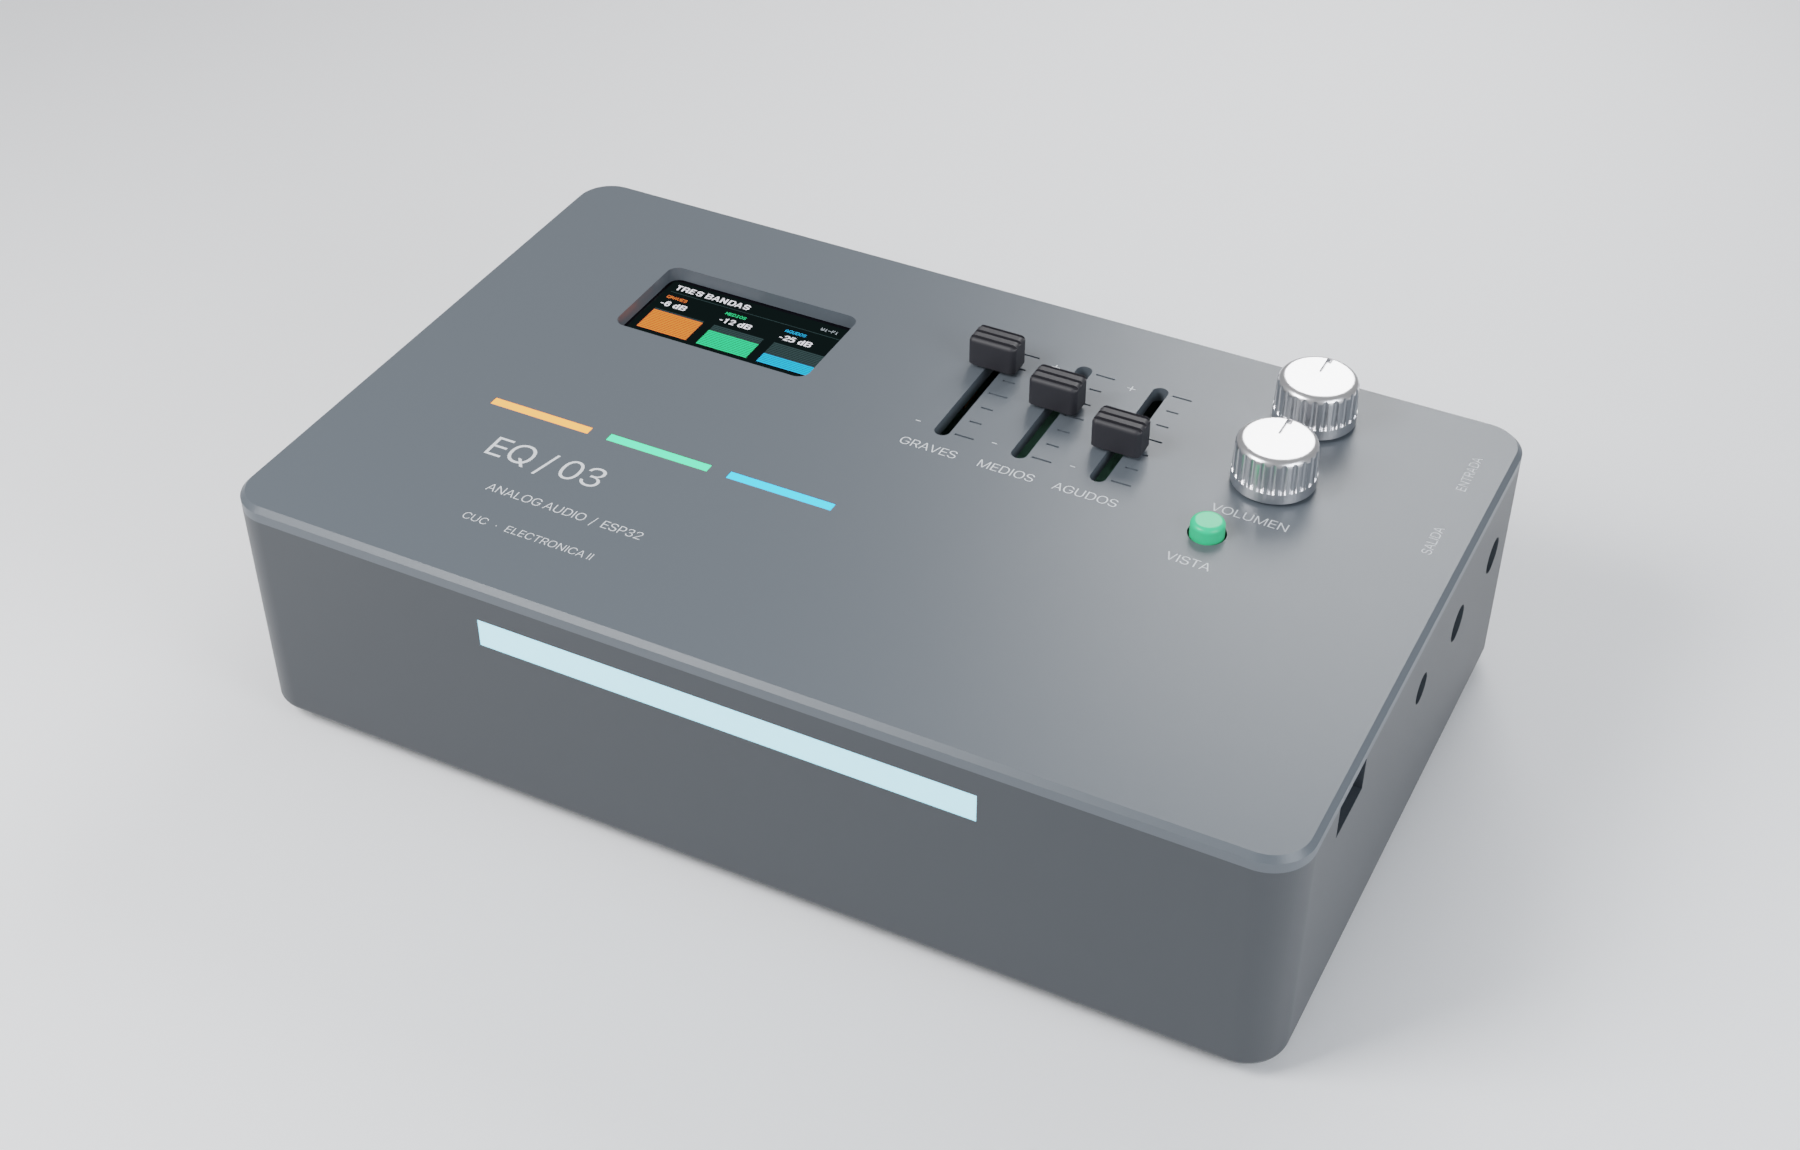
\includegraphics[width=\linewidth,height=5cm,keepaspectratio]{3d-gabinete-cerrado.png}\end{column}\end{columns}
\note{Este es el diseño del ecualizador: el audio pasa por filtros analógicos y el ESP32 muestra sus niveles y espectro. La imagen corresponde al modelo CAD.}
\end{frame}
\begin{frame}[t]{Objetivos del proyecto}
\textbf{Objetivo general}\par Desarrollar un ecualizador de audio de tres bandas que permita ajustar graves, medios y agudos, reproducir la señal procesada y visualizar sus niveles y espectro mediante un ESP32.\vspace{5mm}\par\textbf{Tres objetivos específicos}\begin{enumerate}[<+->]
\item Diseñar los filtros activos y las etapas de ajuste y suma para controlar las tres bandas de audio.
\item Integrar la salida de línea, el amplificador y los controles en un equipo con PCB de una cara y gabinete propio.
\item Programar la adquisición y visualización con el ESP32, y evaluar el equipo mediante simulación y mediciones de laboratorio.
\end{enumerate}
\note{Los objetivos describen las metas del proyecto.}
\end{frame}
\begin{frame}[t]{Antecedentes y decisión de diseño}
\small\textbf{Estado del arte}\par\vspace{2mm}
\begin{tabularx}{\linewidth}{p{36mm}XX}\toprule
Referencia & Aporte & Qué tomamos\\\midrule
Sallen-Key / TI & Filtros activos de segundo orden & Cálculo de los cortes y de $Q$.\\
ADAU1701 / Analog Devices & Procesamiento digital programable & Punto de comparación con la ruta analógica.\\
WLED Audio Reactive & Análisis de audio para iluminación & Referencia de visualización con ESP32.\\\bottomrule\end{tabularx}\par\vspace{7mm}Cada etapa tiene puntos de medida para comparar el montaje con el cálculo.\par\vspace{3mm}\small Fuentes: TI SLOA024B; ficha ADAU1701; documentación WLED.
\note{Los filtros Sallen-Key nos permiten calcular los cortes y medir cada etapa. ADAU1701 resuelve la ecualización con procesamiento digital. WLED aporta una referencia de visualización con ESP32. Conservamos la ruta analógica para trabajar con sus nodos en el laboratorio.}
\end{frame}
\begin{frame}[t]{Materiales principales del prototipo}
\small\begin{tabularx}{\linewidth}{XrX}\toprule
Componente & Cantidad & Función\\\midrule
MCP6004 + zócalos & 4 & 15 unidades activas y una de reserva\\
ESP32-DevKitC V4 & 1 & Adquisición, FFT, pantalla y Wi-Fi\\
Waveshare ST7789V2 de 1,9 pulgadas & 1 & Interfaz 170 × 320\\
Resistencias / condensadores & 32 / 26 & Filtros, acoples y alimentación\\
Potenciómetros / diodos & 5 / 3 & Ajuste y detección de picos\\
74AHCT125 / WS2812B & 1 / 12 LED & Adaptación de datos e iluminación\\
PAM8403 + parlante / fuente 5 V, 3 A & 1 juego & Salida de audio y alimentación\\\bottomrule\end{tabularx}\par\vspace{4mm}
\normalsize Lista por referencia en la BOM. Añadir cables de puente, cables, conectores, caja y tornillería.
\note{Distinguir la lista prevista del inventario ya adquirido. Los 79 componentes del esquema no incluyen todos los elementos externos y mecánicos.}
\end{frame}
\begin{frame}[t]{Recorrido del audio y puntos de medida}
\centering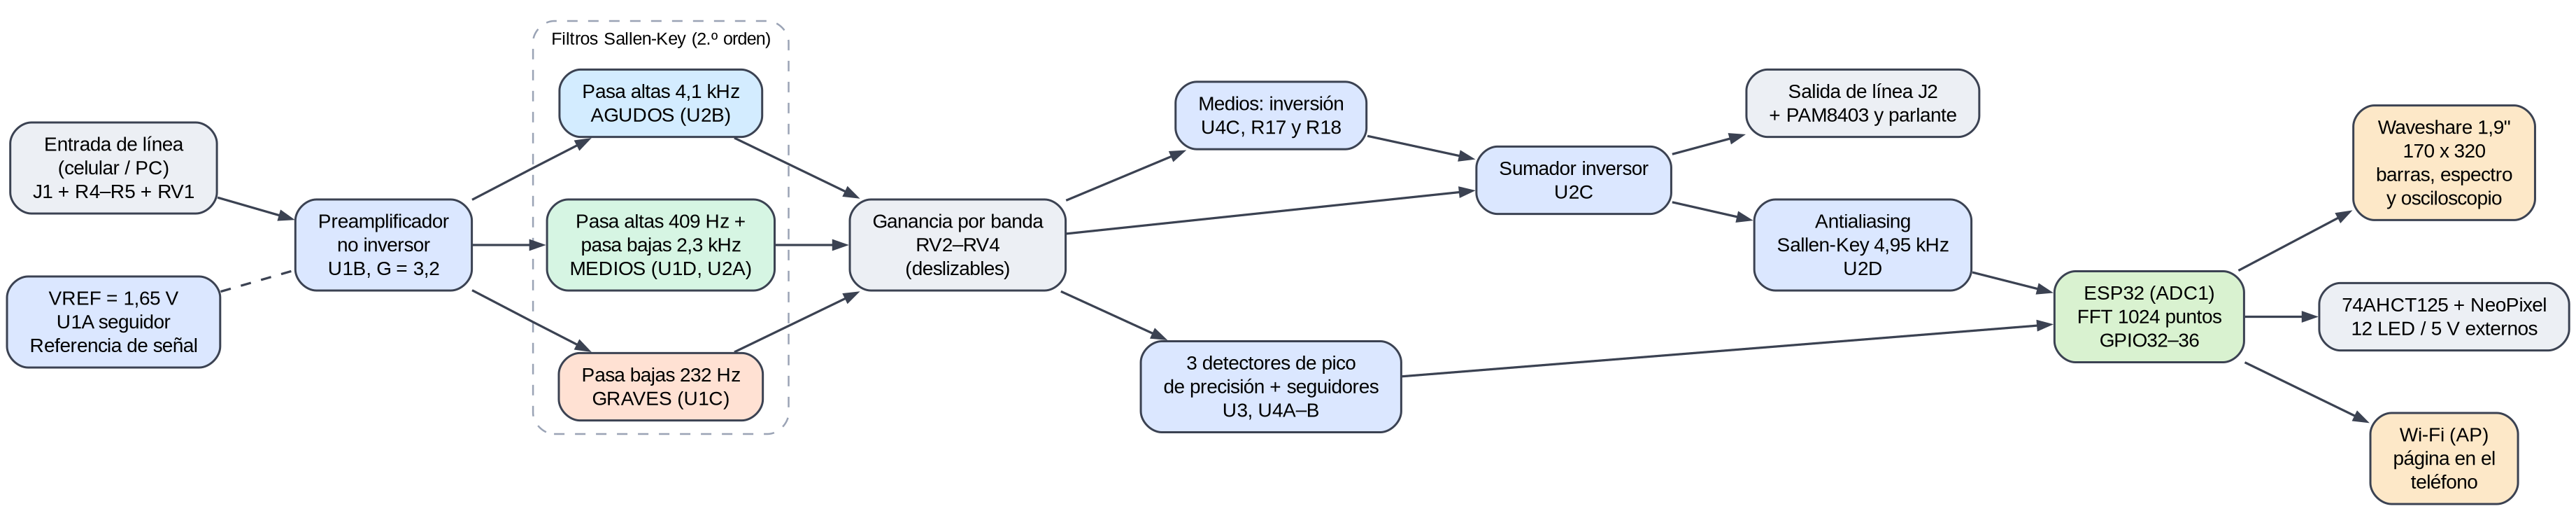
\includegraphics[width=\linewidth,height=4.7cm,keepaspectratio]{diagrama-de-bloques.png}\par\small Entrada de línea $\rightarrow$ filtros y controles $\rightarrow$ salida. El ESP32 observa los detectores y la salida filtrada para la FFT.
\note{Seguir el recorrido del audio de izquierda a derecha. La banda de medios entra invertida al sumador. La iluminación se alimenta desde 5 V y no utiliza VREF como retorno.}
\end{frame}
\begin{frame}[t]{El esquema completo: revisión D.2}
\begin{columns}[T]\begin{column}{.68\textwidth}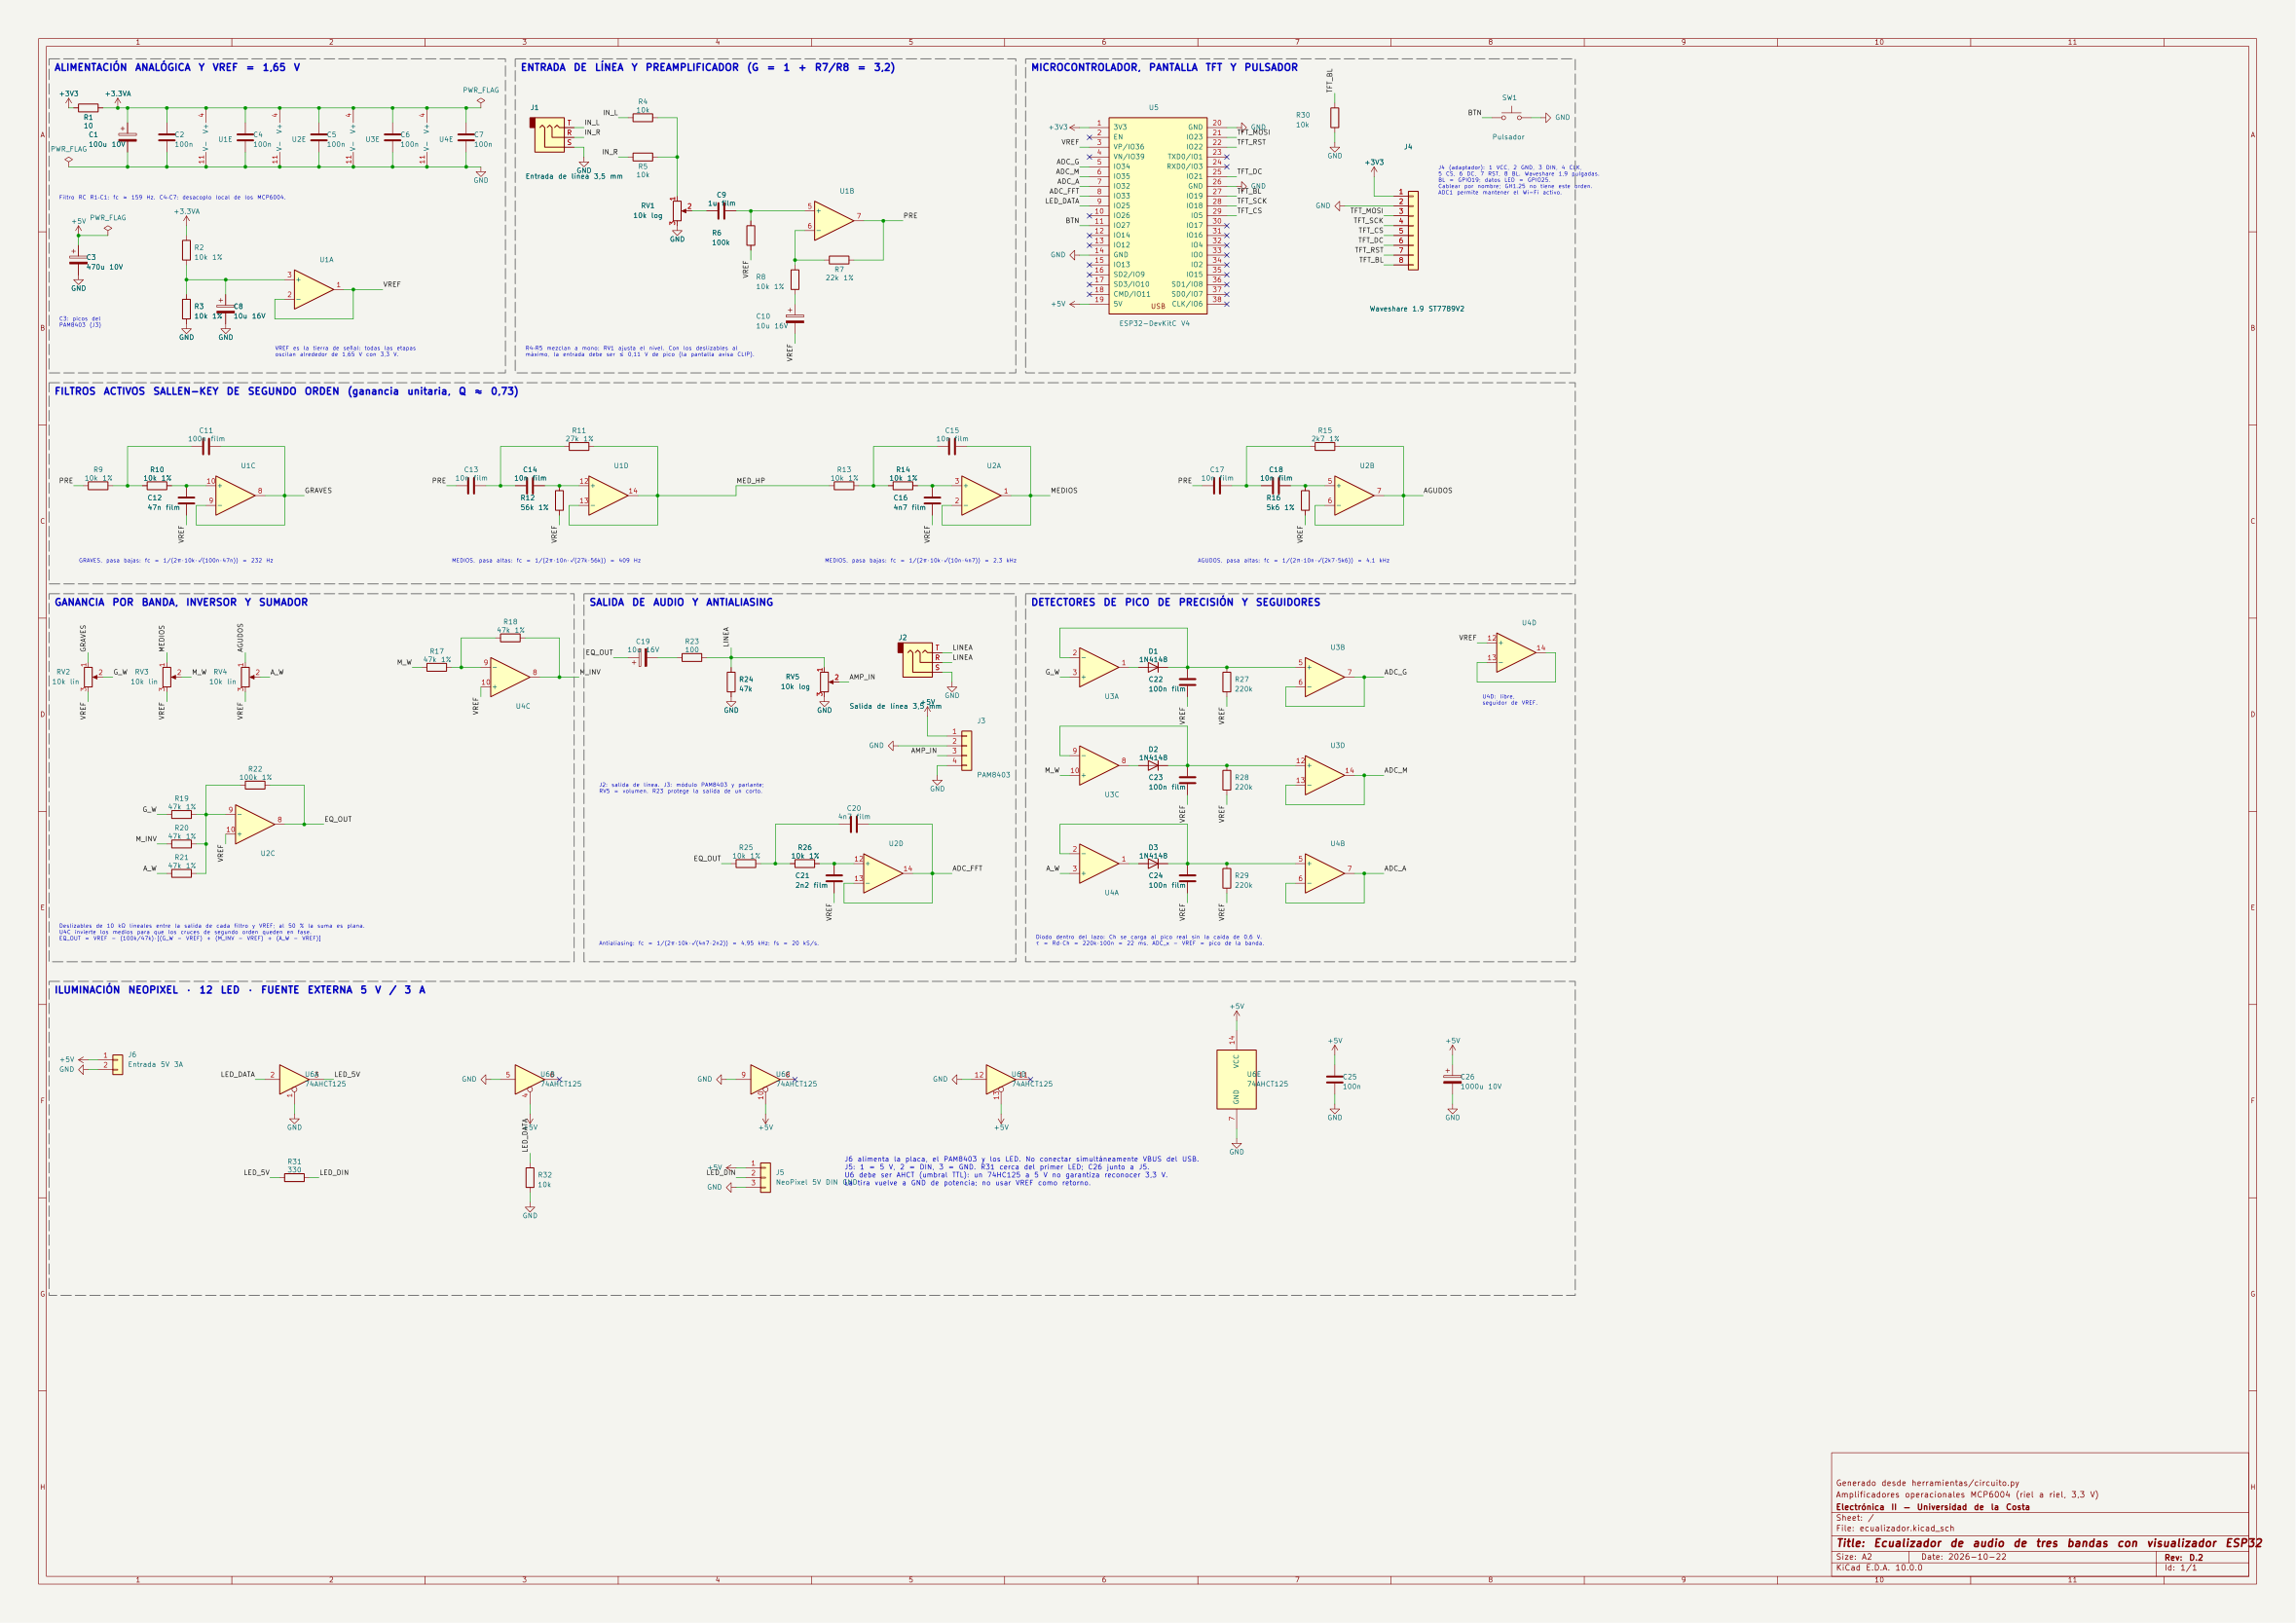
\includegraphics[width=\linewidth,height=5.3cm,keepaspectratio]{esquematico.png}\end{column}\begin{column}{.28\textwidth}\small
Seguir las redes:\par\vspace{3mm}PRE: entrada acondicionada.\par GRAVES / MEDIOS / AGUDOS: filtros.\par EQ\_OUT: suma.\par ADC\_G / M / A: detectores.\par\vspace{4mm}
\hyperlink{esquemacompleto}{\beamergotobutton{Abrir esquema PDF}}
\end{column}\end{columns}
\note{Abrir el PDF vectorial para ampliar los símbolos. El esquema está organizado por etapas y las etiquetas conectan los bloques. VREF es la referencia de audio; GND es el retorno de alimentación.}
\end{frame}
\begin{frame}[t]{Marco teórico: filtros activos Sallen-Key}
\begin{columns}[T]\begin{column}{.56\textwidth}
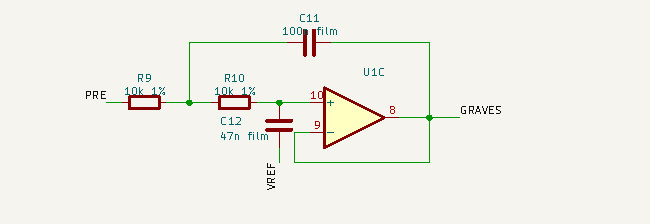
\includegraphics[width=\linewidth,height=3.1cm,keepaspectratio]{circuitos/graves.pdf}
\small U1C: pasa bajas de segundo orden.\\
R9 = R10; C11 realimenta y C12 va a VREF.
\end{column}\begin{column}{.40\textwidth}\small
Para resistencias iguales y ganancia unitaria:
\[
f_0=\frac{1}{2\pi R\sqrt{C_{11}C_{12}}}
\]
\[
Q=\frac12\sqrt{\frac{C_{11}}{C_{12}}}
\]
$f_0$ fija la frecuencia natural; $Q$ determina la forma de la respuesta.
\end{column}\end{columns}\vspace{1mm}
\small El corte a $-3$ dB coincide con $f_0$ cuando $Q=1/\sqrt2$. En medios conectamos un pasa altas y un pasa bajas en cascada.\par
\scriptsize Fuente: Karki, Texas Instruments, SLOA024B. Valores aplicados al esquema del proyecto.
\note{Señalar las dos resistencias, los dos condensadores y el operacional en la figura. La realimentación permite dar forma a la respuesta. No confundir frecuencia natural con corte: nuestros valores comerciales producen Q cercano a 0,73. La banda de medios combina dos secciones de segundo orden y por eso su respuesta completa es de cuarto orden.}
\end{frame}
\begin{frame}[t]{Marco teórico: ajustar y sumar las bandas}
\begin{columns}[T]\begin{column}{.58\textwidth}
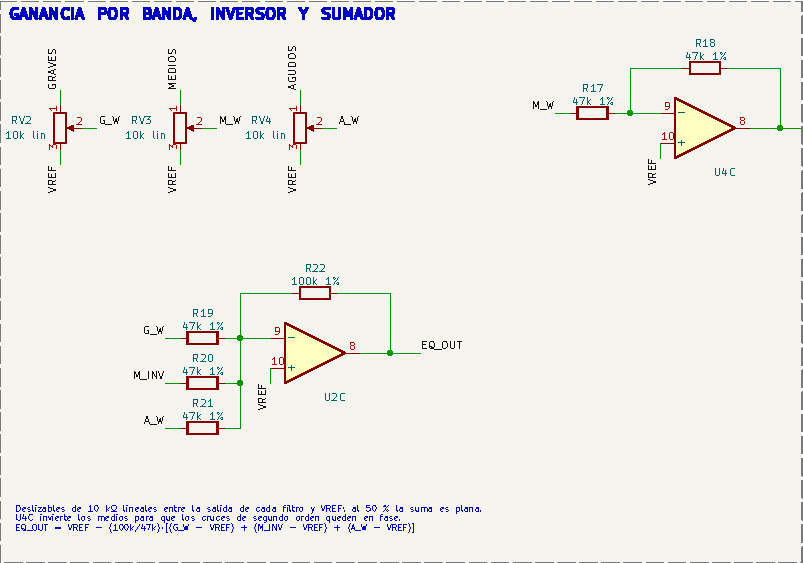
\includegraphics[width=\linewidth,height=4.2cm,keepaspectratio]{circuitos/sumador.pdf}
\end{column}\begin{column}{.38\textwidth}\small
Los deslizables ajustan cuánto aporta cada banda.\par\vspace{3mm}
El sumador combina esas señales con un peso $-R_f/R_i$.\par\vspace{3mm}
U4C invierte medios antes de sumarlos. La fase influye en el resultado.
\end{column}\end{columns}
\small Todas las señales se expresan respecto a VREF: $v_x=V_x-V_{REF}$.
\[
v_{EQ}=-\frac{100}{47}\left(v_{G_W}+v_{M_{INV}}+v_{A_W}\right)
\]
\note{Esta ecuación describe el circuito con alimentación única: primero restamos la referencia de 1,65 voltios. El signo menos corresponde al sumador inversor. La rama de medios ya llega invertida por U4C. Al mover un deslizable cambia la contribución de esa banda; la respuesta total depende también de las fases. La salida de línea entrega la señal al amplificador de potencia que mueve el parlante.}
\end{frame}
\begin{frame}[t]{3,3 V de alimentación; 1,65 V de referencia}
\begin{columns}[T]\begin{column}{.66\textwidth}
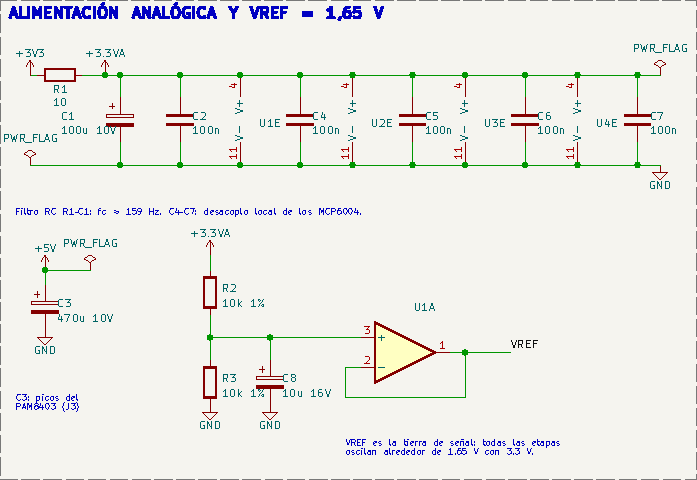
\includegraphics[width=\linewidth,height=4.9cm,keepaspectratio]{circuitos/referencia.pdf}
\end{column}\begin{column}{.30\textwidth}\small
R2 y R3 dividen la alimentación. U1A entrega VREF a los filtros.\par\vspace{4mm}
Filtro RC: R1 y C1.\par Desacoplo: C2 y C4–C7.\par\vspace{4mm}
En reposo: 1,641 V simulados.\par\vspace{4mm}
LED y alimentación del PAM8403: retorno a GND. El parlante va entre las dos salidas BTL.
\end{column}\end{columns}
\note{El audio oscila alrededor de VREF porque usamos una alimentación de 3,3 V. U1A evita cargar directamente el divisor. La caída en R1 deja la referencia en 1,641 V en la simulación. U1E es la unidad de alimentación de U1, no otro operacional. PWR\_FLAG es una marca para ERC; no se compra.}
\end{frame}
\begin{frame}[t]{Entrada y ganancia del preamplificador}
\begin{columns}[T]\begin{column}{.66\textwidth}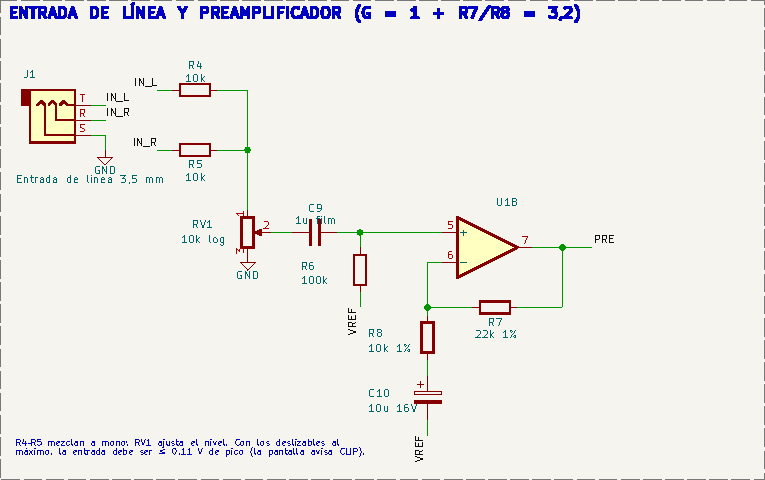
\includegraphics[width=\linewidth,height=5cm,keepaspectratio]{circuitos/entrada.pdf}\end{column}\begin{column}{.30\textwidth}\small
\textbf{R4 y R5}\par Mezclan L/R sin unir directamente las salidas de la fuente.\par\vspace{3mm}
\textbf{RV1, C9 y R6}\par Ajustan nivel, bloquean continua y polarizan en VREF.\par\vspace{3mm}
\textbf{U1B, R7 y R8}\par Ganancia de 3,2 en banda. C10 deja ganancia unitaria en continua.
\end{column}\end{columns}
\note{R4 y R5 mezclan los canales del jack; RV1 ajusta cuánto llega al preamplificador. C9 bloquea la continua y R6 centra la señal en VREF. La ganancia de 3,2 se comprueba entre PRE\_IN y PRE. Si la entrada es demasiado grande, el operacional satura.}
\end{frame}
\begin{frame}[t]{Filtro de graves: U1C, R9, R10, C11 y C12}
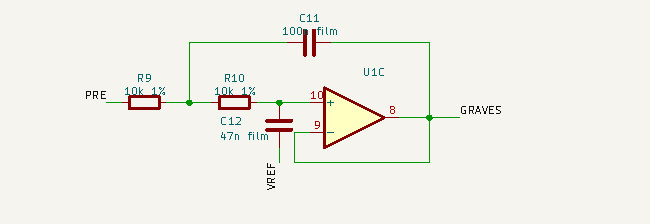
\includegraphics[width=.86\linewidth,height=3.3cm,keepaspectratio]{circuitos/graves.pdf}\par\vspace{3mm}
\begin{columns}[T]\begin{column}{.48\textwidth}\small
R9 = R10 = 10 k$\Omega$.\par C11 = 100 nF; C12 = 47 nF.\par U1C trabaja como seguidor.\end{column}\begin{column}<2->{.48\textwidth}\small
C11 vuelve desde la salida al nodo intermedio. C12 deriva a VREF.\par La realimentación fija $Q\approx0,73$; el corte simulado es 239 Hz.
\end{column}\end{columns}
\note{A baja frecuencia los condensadores cargan poco la señal; a alta frecuencia aumenta su efecto y cae la salida de graves. El filtro no es solo dos RC independientes: C11 realimenta desde la salida. Medios encadena pasa altas y pasa bajas; agudos usa pasa altas.}
\end{frame}
\begin{frame}[t]{Medios: dos filtros conectados en cascada}
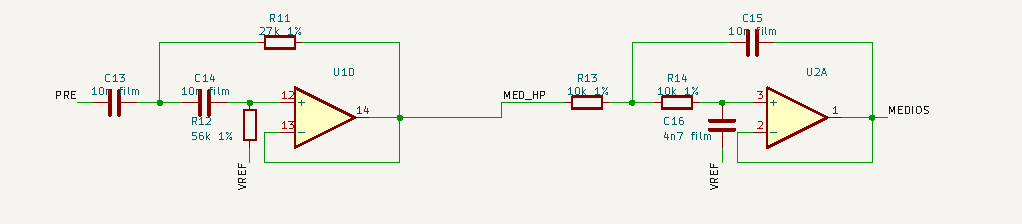
\includegraphics[width=\linewidth,height=3.1cm,keepaspectratio]{circuitos/medios.pdf}\par\vspace{4mm}
\begin{columns}[T]\begin{column}{.48\textwidth}\small
U1D: pasa altas de 403 Hz.\par C13 = C14 = 10 nF.\par R11 = 27 k$\Omega$; R12 = 56 k$\Omega$.
\end{column}\begin{column}<2->{.48\textwidth}\small
U2A: pasa bajas de 2388 Hz.\par R13 = R14 = 10 k$\Omega$.\par C15 = 10 nF; C16 = 4,7 nF.
\end{column}\end{columns}
\note{La salida de U1D entra directamente a U2A por MED\_HP. El primer filtro atenúa los graves y el segundo atenúa los agudos. Entre ambos queda la banda de medios. Son dos secciones de segundo orden conectadas en cascada.}
\end{frame}
\begin{frame}[t]{Agudos: pasa altas con U2B}
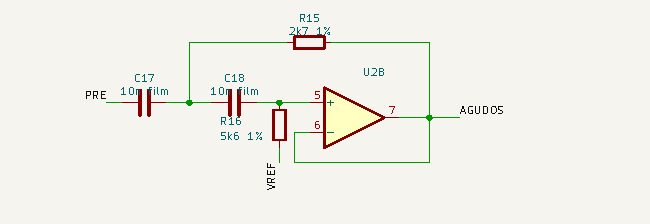
\includegraphics[width=.88\linewidth,height=3.4cm,keepaspectratio]{circuitos/agudos.pdf}\par\vspace{3mm}
\begin{columns}[T]\begin{column}{.48\textwidth}\small
C17 = C18 = 10 nF.\par R15 = 2,7 k$\Omega$; R16 = 5,6 k$\Omega$.
\end{column}\begin{column}<2->{.48\textwidth}\small
Corte simulado: 4026 Hz.\par La salida llega a RV4, que regula su aporte a la mezcla.
\end{column}\end{columns}
\note{Los condensadores están en serie con la señal. A baja frecuencia atenúan la entrada; por encima del corte aumenta la salida de agudos. U2B trabaja como seguidor dentro del filtro.}
\end{frame}
\begin{frame}[t]{Frecuencias calculadas y simuladas}
\begin{center}\begin{tabular}{lrr}\toprule
Filtro & Cálculo de $f_0$ & Corte simulado\\\midrule
Graves (U1C), pasa bajas & 232 Hz & 239 Hz\\
Medios (U1D), pasa altas & 409 Hz & 403 Hz\\
Medios (U2A), pasa bajas & 2322 Hz & 2388 Hz\\
Agudos (U2B), pasa altas & 4093 Hz & 4026 Hz\\
Previo al ADC (U2D) & 4949 Hz & 5101 Hz\\\bottomrule\end{tabular}\end{center}\vspace{3mm}\[ f_{0,PB}=\frac{1}{2\pi R\sqrt{C_1C_2}}\qquad f_{0,PA}=\frac{1}{2\pi C\sqrt{R_1R_2}}\]\small Cada sección es de segundo orden. La cascada de medios es de cuarto orden.
\note{Distinguir frecuencia natural y corte a menos tres decibelios: con Q cercano a 0,73 no coinciden exactamente. Todos los cortes nominales simulados cumplen el margen del diez por ciento.}
\end{frame}
\begin{frame}[t]{Deslizables, inversión de medios y sumador}
\begin{columns}[T]\begin{column}{.64\textwidth}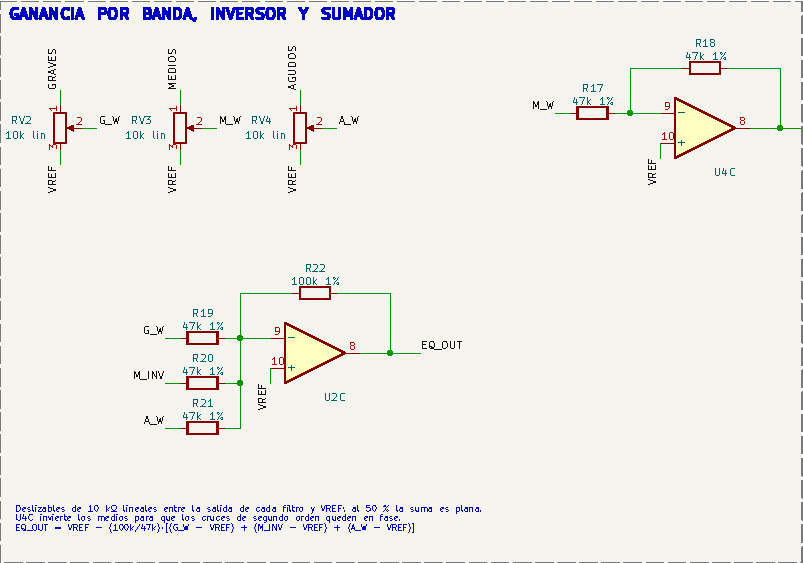
\includegraphics[width=\linewidth,height=5.2cm,keepaspectratio]{circuitos/sumador.pdf}\end{column}\begin{column}{.32\textwidth}\small
RV2--RV4 entregan una fracción de cada banda respecto a VREF.\par\vspace{4mm}
U4C invierte medios: $-47/47=-1$.\par\vspace{4mm}
U2C suma por R19--R21. Cada entrada pesa $-100/47\approx-2,13$.\par\vspace{4mm}
La fase de cada banda también afecta la suma.
\end{column}\end{columns}
\note{Cada deslizable entrega una fracción de su banda al sumador. U4C invierte medios antes de la suma. Al simular la cadena completa, esta corrección reduce los valles en los cruces; la siguiente curva muestra la comparación.}
\end{frame}
\begin{frame}[t]{Respuesta de la suma antes y después de corregir la fase}
\centering\only<1|handout:0>{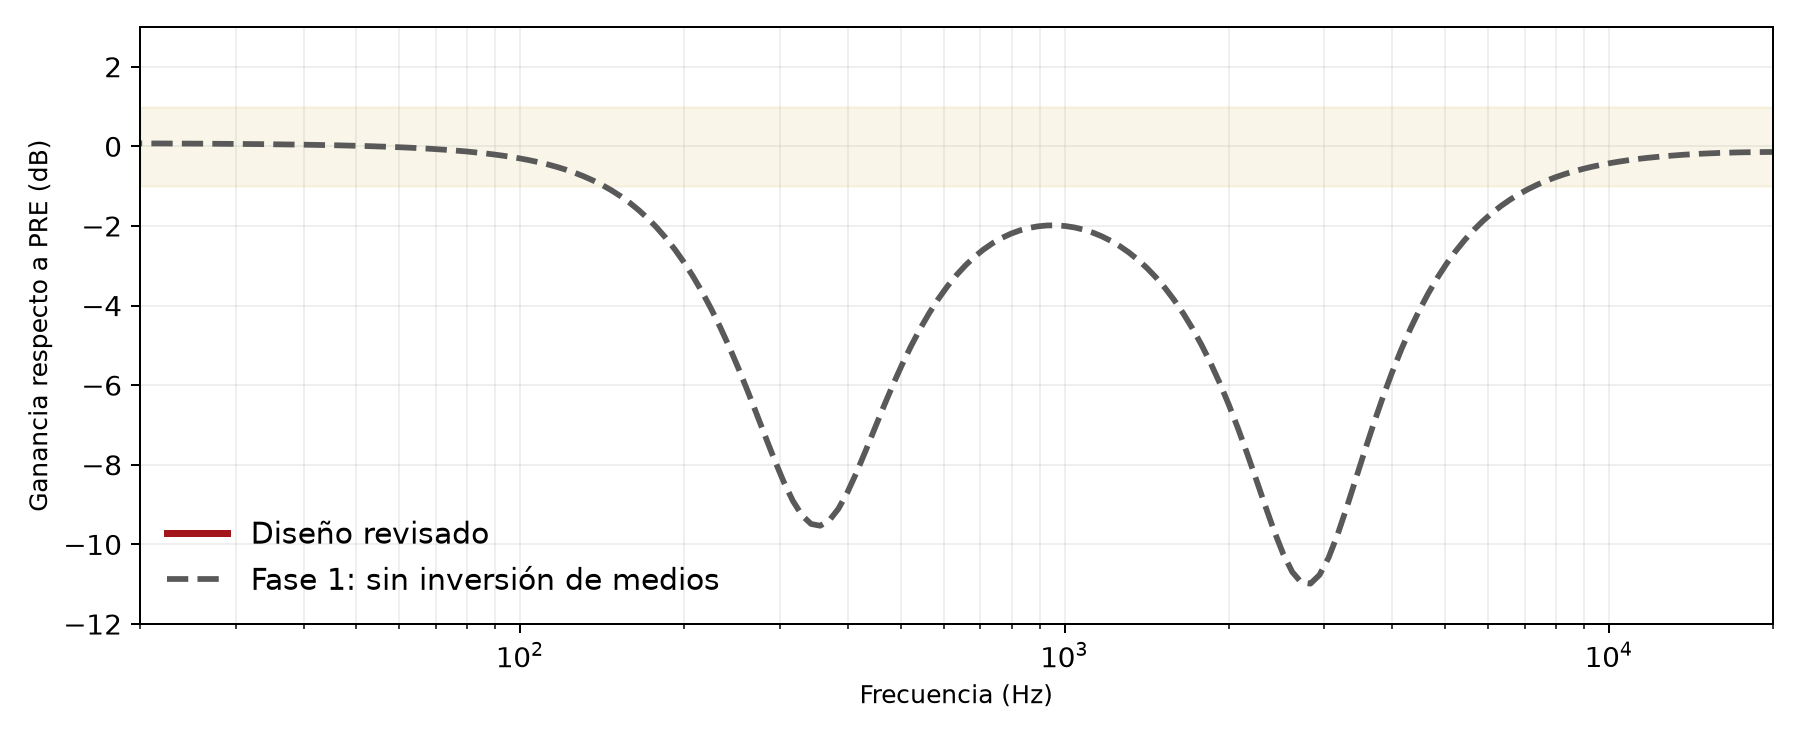
\includegraphics[width=\linewidth,height=4.9cm,keepaspectratio]{sim-comparacion-fase-inicial.png}}%
\only<2|handout:1>{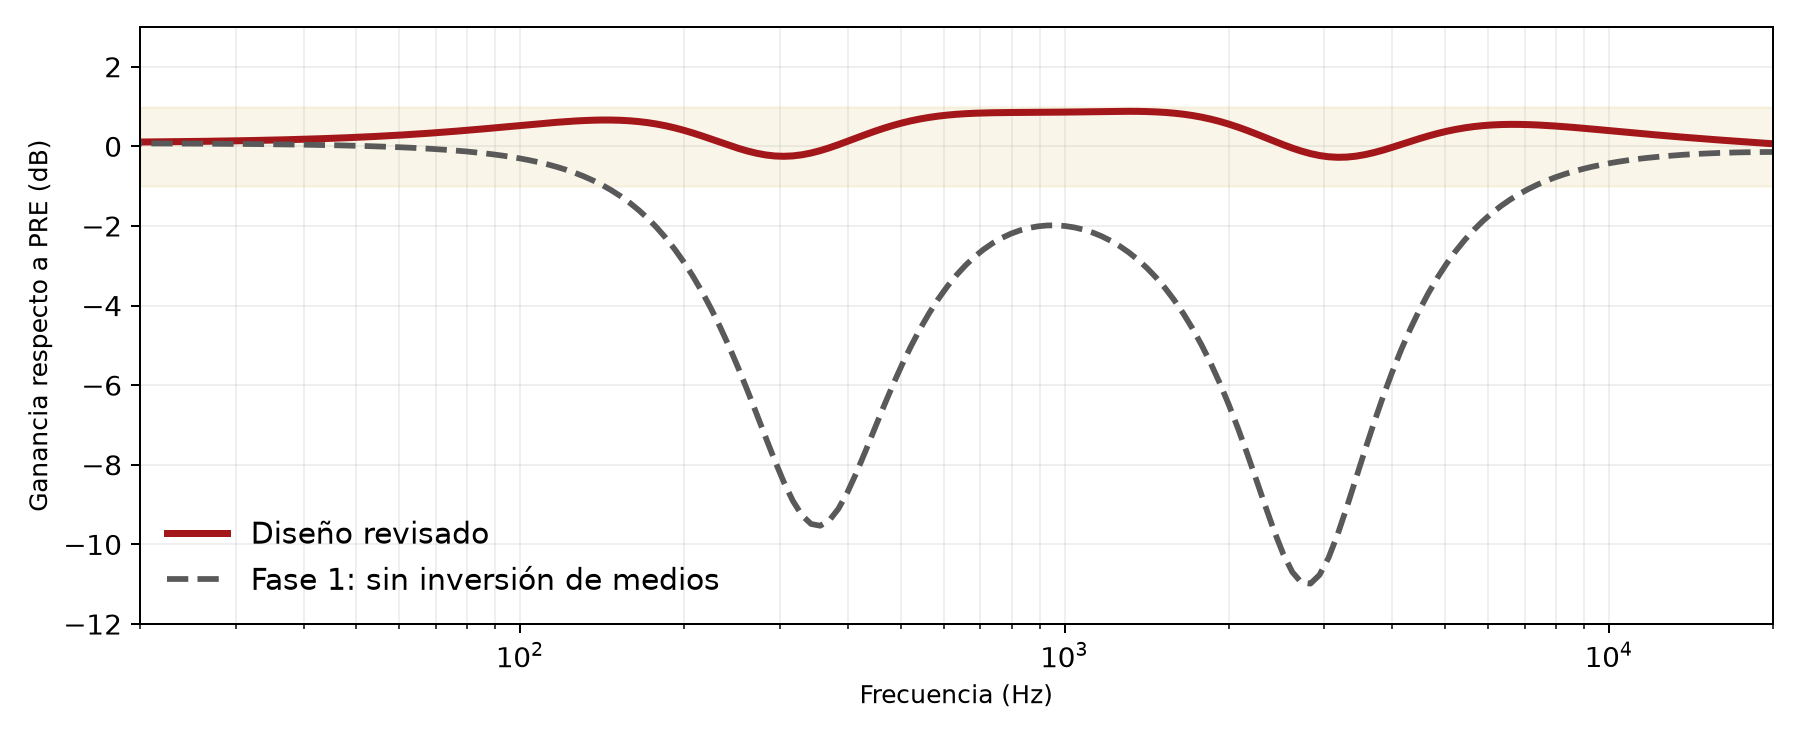
\includegraphics[width=\linewidth,height=4.9cm,keepaspectratio]{sim-comparacion-fase.png}}\par\small U4C, R17 y R18 corrigen la fase de medios. Al centro: de $-11$ dB a una respuesta entre $-0,27$ y $+0,88$ dB respecto a PRE.
\note{Explicar la inversión de medios con U4C y el reajuste de sus cortes. La curva corresponde a ngspice y a un modelo aproximado, no a mediciones del equipo. No llamar a este diseño un cruce Linkwitz-Riley exacto.}
\end{frame}
\begin{frame}[t]{Detector de pico y seguidor para el ADC}
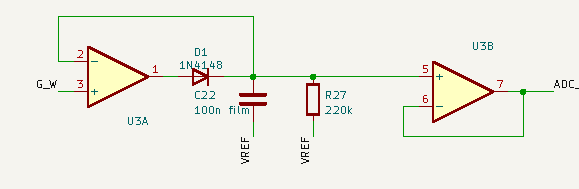
\includegraphics[width=\linewidth,height=3cm,keepaspectratio]{circuitos/detector-graves.pdf}\par\vspace{5mm}
\begin{columns}[T]\begin{column}{.48\textwidth}\small
\textbf{U3A + D2}\par Cargan C22 durante los picos positivos. El diodo queda dentro de la realimentación.\end{column}\begin{column}<2->{.48\textwidth}\small
\textbf{R27 + C22 + U3B}\par Descarga de 22 ms y seguidor para el ADC. Se resta VREF para obtener el nivel de graves.
\end{column}\end{columns}
\note{El detector entrega una envolvente con rizado, no un RMS. La compensación del diodo es una aproximación limitada por la velocidad, saturación y recuperación del operacional. A frecuencias bajas hay más descarga entre picos.}
\end{frame}
\begin{frame}[t]{Niveles de los detectores con un tono de 1 kHz}
\begin{columns}[T]\begin{column}{.43\textwidth}\textbf{Tono de 1 kHz}\par\vspace{4mm}\begin{tabular}{lr}Graves & 15 mV\\Medios & 304 mV\\Agudos & 17 mV\end{tabular}\vspace{6mm}\par\[\tau=220\,\mathrm{k}\Omega\cdot100\,\mathrm{nF}=22\,\mathrm{ms}\]\small D2 a D3, C22 a C24 y R27 a R29.\par La lectura corresponde a la envolvente.\end{column}\begin{column}{.54\textwidth}\centering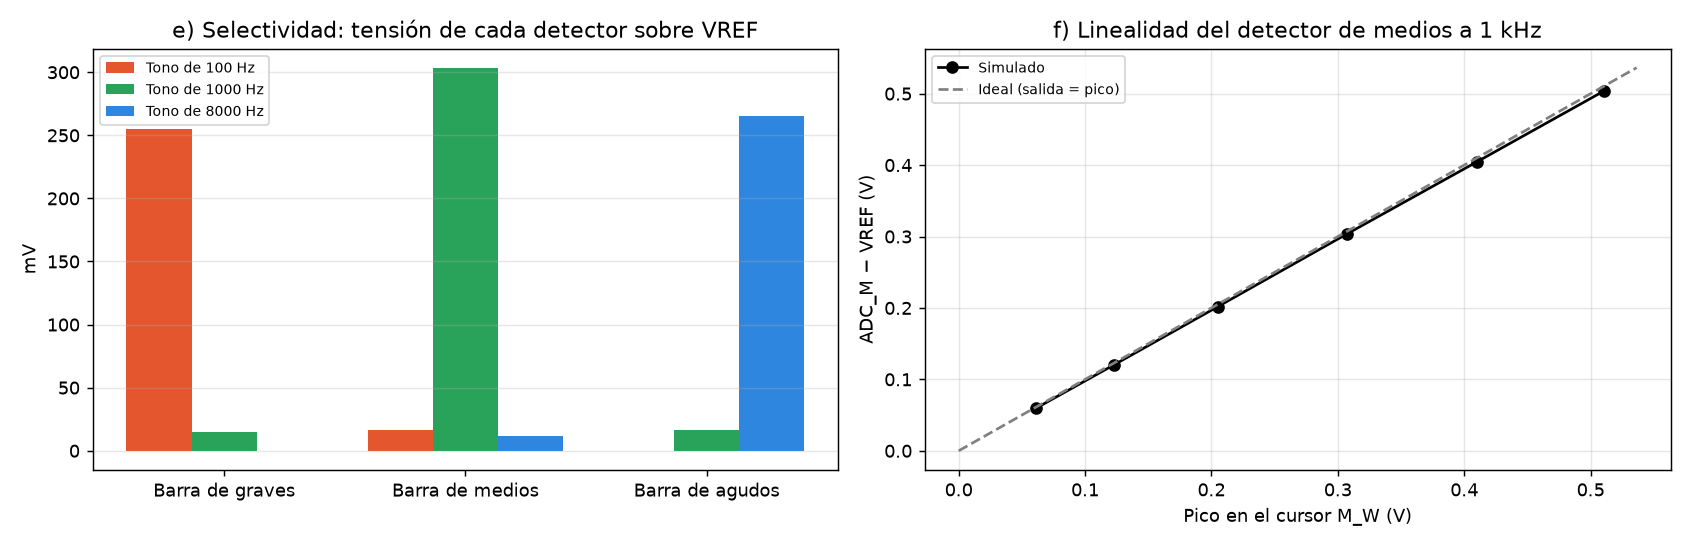
\includegraphics[width=\linewidth,height=5cm,keepaspectratio]{sim-detectores.png}\end{column}\end{columns}
\note{Las lecturas son las tensiones del detector menos VREF. El criterio de selectividad es una relación de al menos cuatro a uno. La descarga entre picos afecta más a frecuencias bajas.}
\end{frame}
\begin{frame}[t]{Antes de la FFT: filtro y entrada al ADC}
\begin{columns}[T]\begin{column}{.64\textwidth}
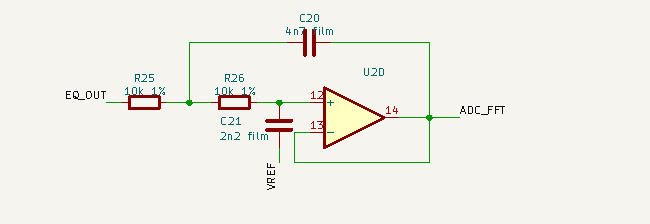
\includegraphics[width=\linewidth,height=4.8cm,keepaspectratio]{circuitos/antialias.pdf}
\end{column}\begin{column}{.32\textwidth}\small
U2D, R25 y R26 de 10 k$\Omega$.\par C20 = 4,7 nF; C21 = 2,2 nF.\par\vspace{4mm}
ADC\_FFT llega a GPIO33.\par Corte simulado: 5101 Hz.\par\vspace{4mm}
A 15 kHz atenúa 19,3 dB. Una señal fuerte todavía puede producir aliasing.
\end{column}\end{columns}
\note{Este filtro está después del sumador y antes del ADC. Reduce las componentes por encima de la zona que queremos visualizar. Con 20 mil muestras por segundo, un tono de 15 kHz puede plegarse a 5 kHz si no queda suficientemente atenuado.}
\end{frame}
\begin{frame}[t]{Muestreo y resolución de la FFT}
\begin{columns}[T]\begin{column}{.47\textwidth}
{\Huge 1024}\par muestras por bloque\vspace{5mm}\par $f_s=20$ kS/s\par $\Delta f=19,53$ Hz\par Tiempo de bloque: 51,2 ms\end{column}\begin{column}<2->{.49\textwidth}
\textbf{Un tono de 1 kHz}\par queda cerca del bin 51 (996,1 Hz).\vspace{5mm}\par\textbf{Límite del análisis}\par Se muestran aproximadamente 40 Hz--5 kHz. El filtro atenúa el aliasing; no lo elimina.\vspace{3mm}\par\small U2D entrega la señal a GPIO33 de U5.\par A 15 kHz: $-19,3$ dB simulados.\end{column}\end{columns}
\note{La frecuencia que muestra el estimador interpolado puede acercarse a mil hertz. El muestreo nominal y los cinco cuadros por segundo se deben medir en la placa con Wi-Fi activo.}
\end{frame}
\begin{frame}[t]{Pantalla: conexión SPI y control de luz}
\begin{columns}[T]\begin{column}{.66\textwidth}
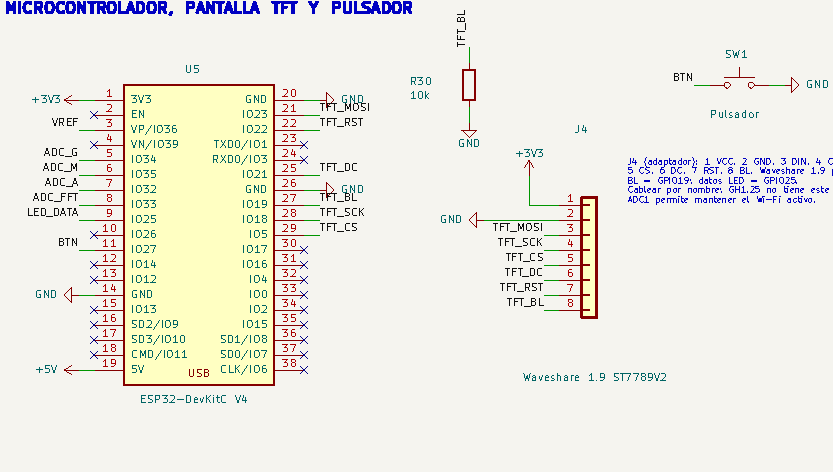
\includegraphics[width=\linewidth,height=5cm,keepaspectratio]{circuitos/pantalla.pdf}
\end{column}\begin{column}{.30\textwidth}\small
U5: ESP32-DevKitC.\par J4: cable de ocho señales.\par\vspace{4mm}
DIN y CLK llevan los datos. CS, DC y RST controlan la pantalla.\par\vspace{4mm}
GPIO19 controla BL; R30 lo mantiene apagado al arrancar.
\end{column}\end{columns}
\note{La pantalla Waveshare se conecta por cable y queda sujeta a la tapa. J4 usa paso de 2,54 mm; el módulo usa GH1.25. El adaptador se revisa por nombre de señal porque los números de ambos conectores no coinciden.}
\end{frame}
\begin{frame}[t]{Waveshare 1,9 pulgadas · 170 × 320}
\begin{columns}[T]\begin{column}{.43\textwidth}\textbf{ST7789V2 por SPI}\par En horizontal: 320 × 170.\vspace{4mm}\par Módulo: 51,2 × 27,3 mm.\par Área activa: 42,72 × 22,70 mm.\vspace{4mm}\par J4 usa un cable adaptador de 8 señales.\par\small Verificar el orden por nombre; el conector del módulo es GH1.25.\end{column}\begin{column}{.54\textwidth}\centering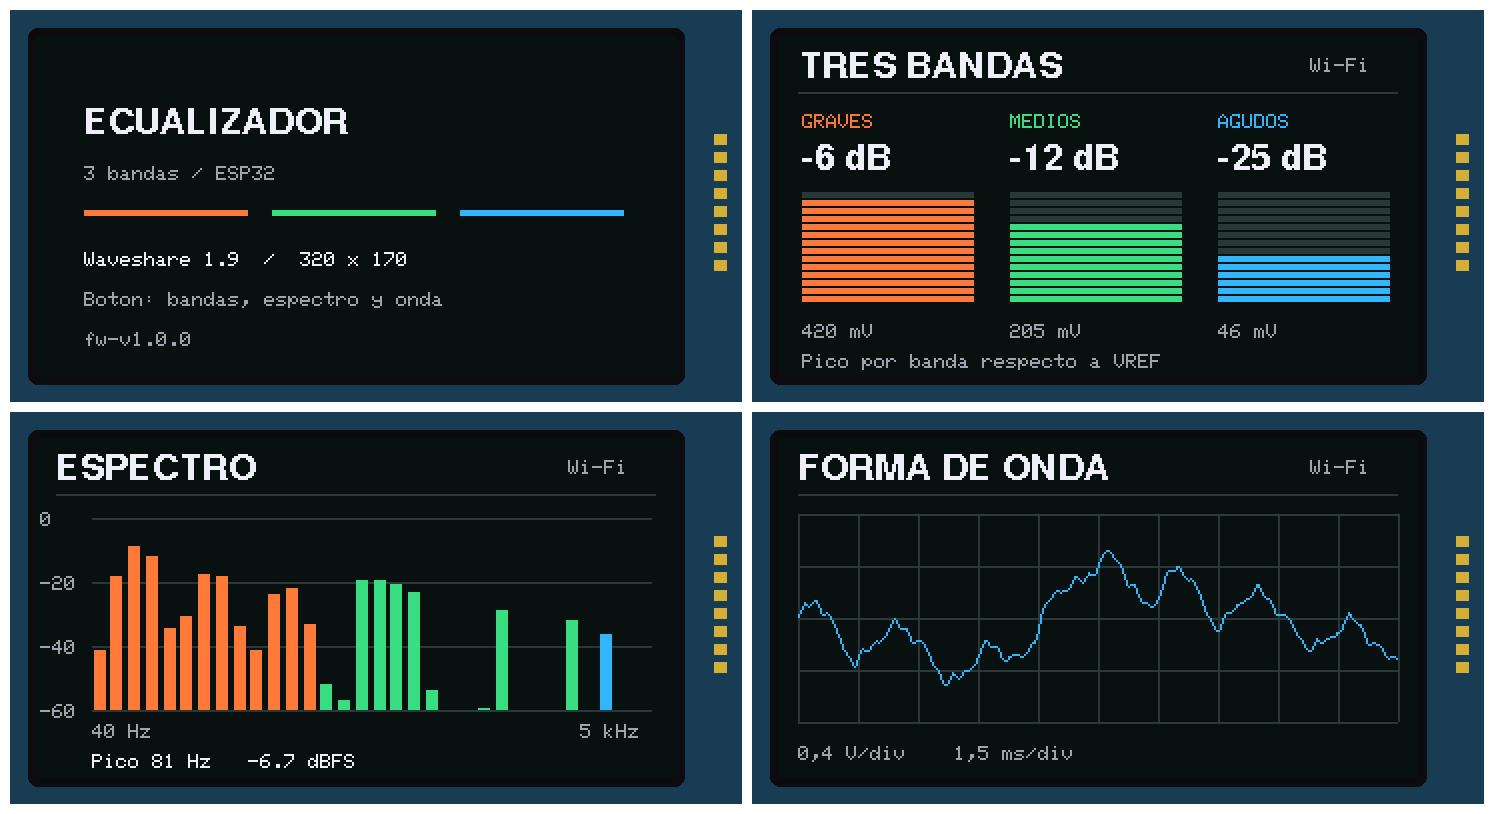
\includegraphics[width=\linewidth,height=5cm,keepaspectratio]{ui-tft-vistas.png}\end{column}\end{columns}
\note{Las imágenes salen del código de interfaz usando datos de ejemplo. No son fotografías de la pantalla real. El controlador nuevo y la altura reducida ya están integrados en el firmware.}
\end{frame}
\begin{frame}[t]{Circuito de alimentación y datos de los LED}
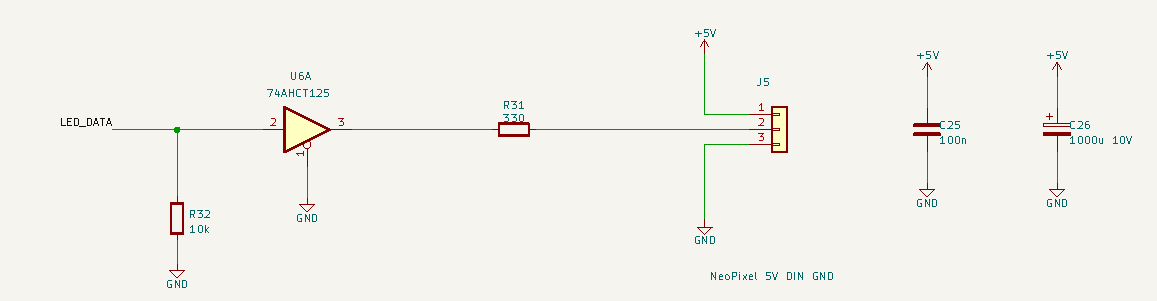
\includegraphics[width=\linewidth,height=3.7cm,keepaspectratio]{circuitos/neopixel.pdf}\par\vspace{3mm}
\small U6: 74AHCT125 a 5 V. R31: 330 $\Omega$ en DIN. C25: 100 nF. C26: 1000 $\mu$F.\par
J5 conecta la tira; J6 recibe la fuente de 5 V / 3 A. R32 mantiene los datos bajos durante el arranque.
\note{GPIO25 entrega 3,3 V y U6 adapta la señal a 5 V. Usamos AHCT por su umbral de entrada TTL. La tira comparte GND con el controlador. Al usar la fuente externa se desconecta VBUS del USB.}
\end{frame}
\begin{frame}[t]{NeoPixel: canal, difusor y alimentación}
\begin{columns}[T]\begin{column}{.43\textwidth}Dos tramos de 100 mm: \textbf{12 LED}.\par\vspace{3mm}Canales interiores de\par102 × 10,6 × 3 mm.\par\vspace{3mm}GPIO25 $\rightarrow$ 74AHCT125\par$\rightarrow$ 330 $\Omega$ $\rightarrow$ DIN.\par\vspace{3mm}Fuente externa 5 V / 3 A.\par1000 $\mu$F de reserva.\par\vspace{3mm}\small Brillo inicial 32/255; iluminación fija y tenue.\end{column}\begin{column}<2->{.54\textwidth}\centering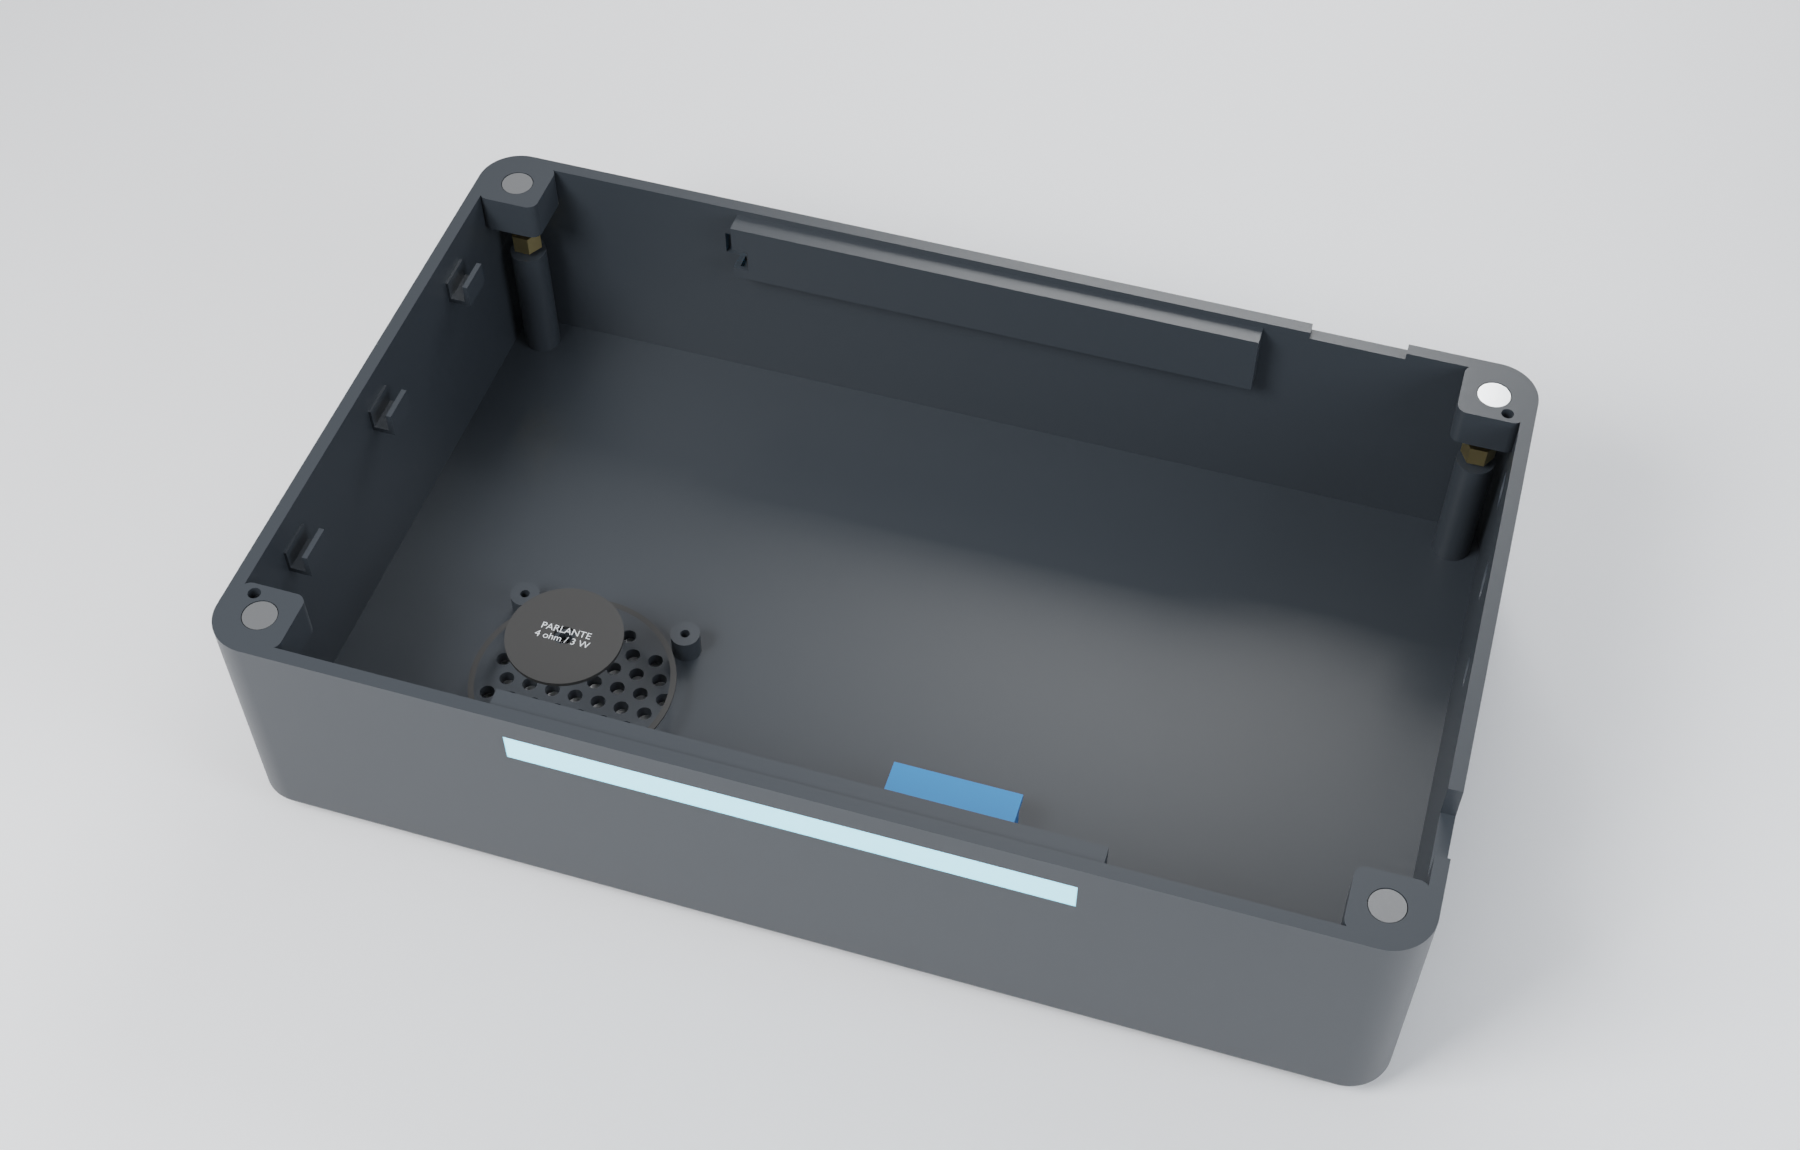
\includegraphics[width=\linewidth,height=5cm,keepaspectratio]{3d-gabinete-canales.png}\end{column}\end{columns}
\note{La tira no se alimenta desde 3,3 V. El 74AHCT125 adapta el nivel de datos. La reserva de corriente se dimensiona hasta 720 mA para los LED, aunque el firmware limita el brillo. Con fuente externa no se conecta VBUS del USB.}
\end{frame}
\begin{frame}[t]{Esquemático y PCB: comprobaciones distintas}
\begin{columns}[T]\begin{column}{.43\textwidth}\textbf{Esquemático}\par ERC: 0 errores, 0 advertencias.\par 59 redes coinciden pin a pin.\vspace{5mm}\par\textbf{PCB}\par Una cara, 200 × 120 mm.\par Cobre por debajo y 80 puentes aislados.\vspace{4mm}\par\small DRC: 0 errores, 0 conexiones abiertas.\end{column}\begin{column}{.54\textwidth}\centering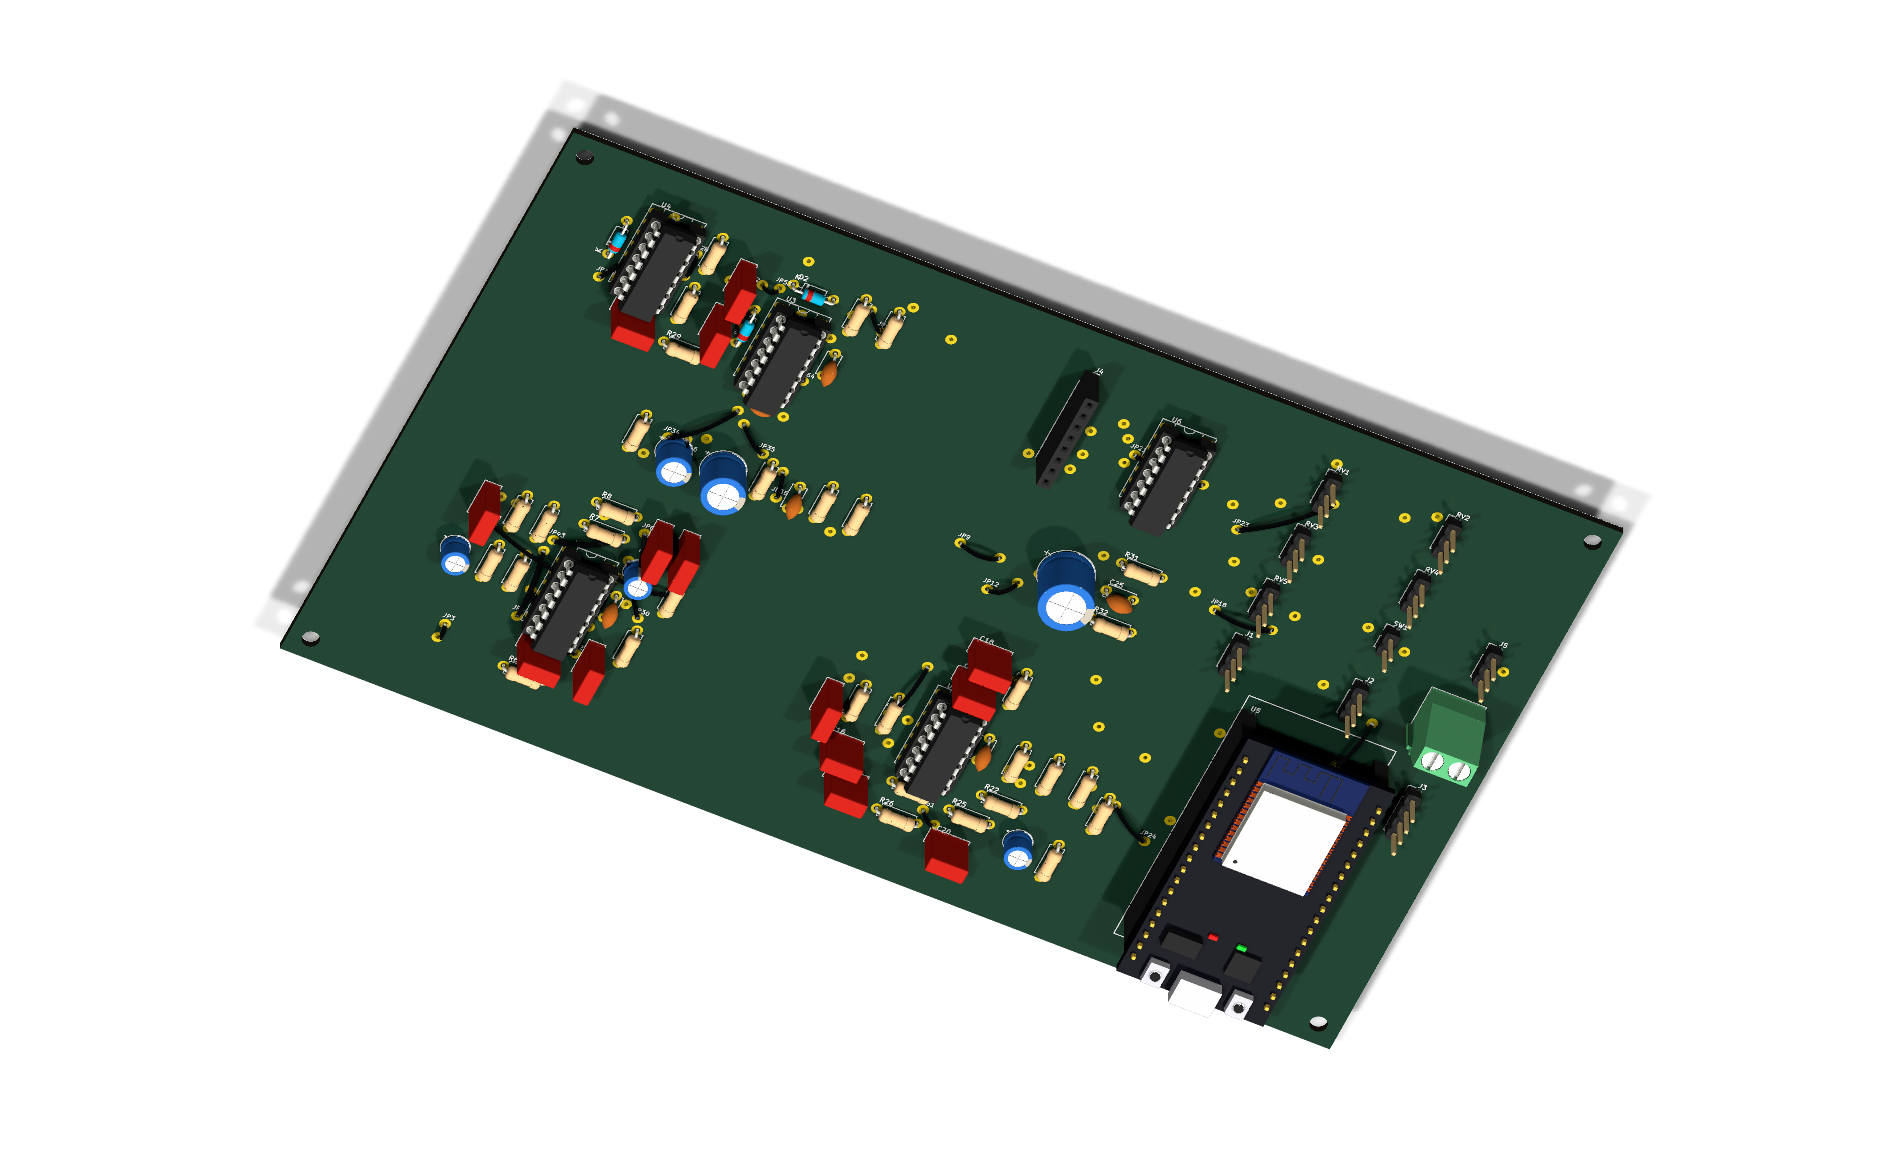
\includegraphics[width=\linewidth,height=5cm,keepaspectratio]{3d-placa-iso.png}\end{column}\end{columns}
\note{ERC comprueba el esquema y DRC comprueba la placa. La continuidad incluye los 80 cables.}
\end{frame}
\begin{frame}[t]{D.2: PCB de una cara con puentes}
\begin{columns}[T]\begin{column}{.69\textwidth}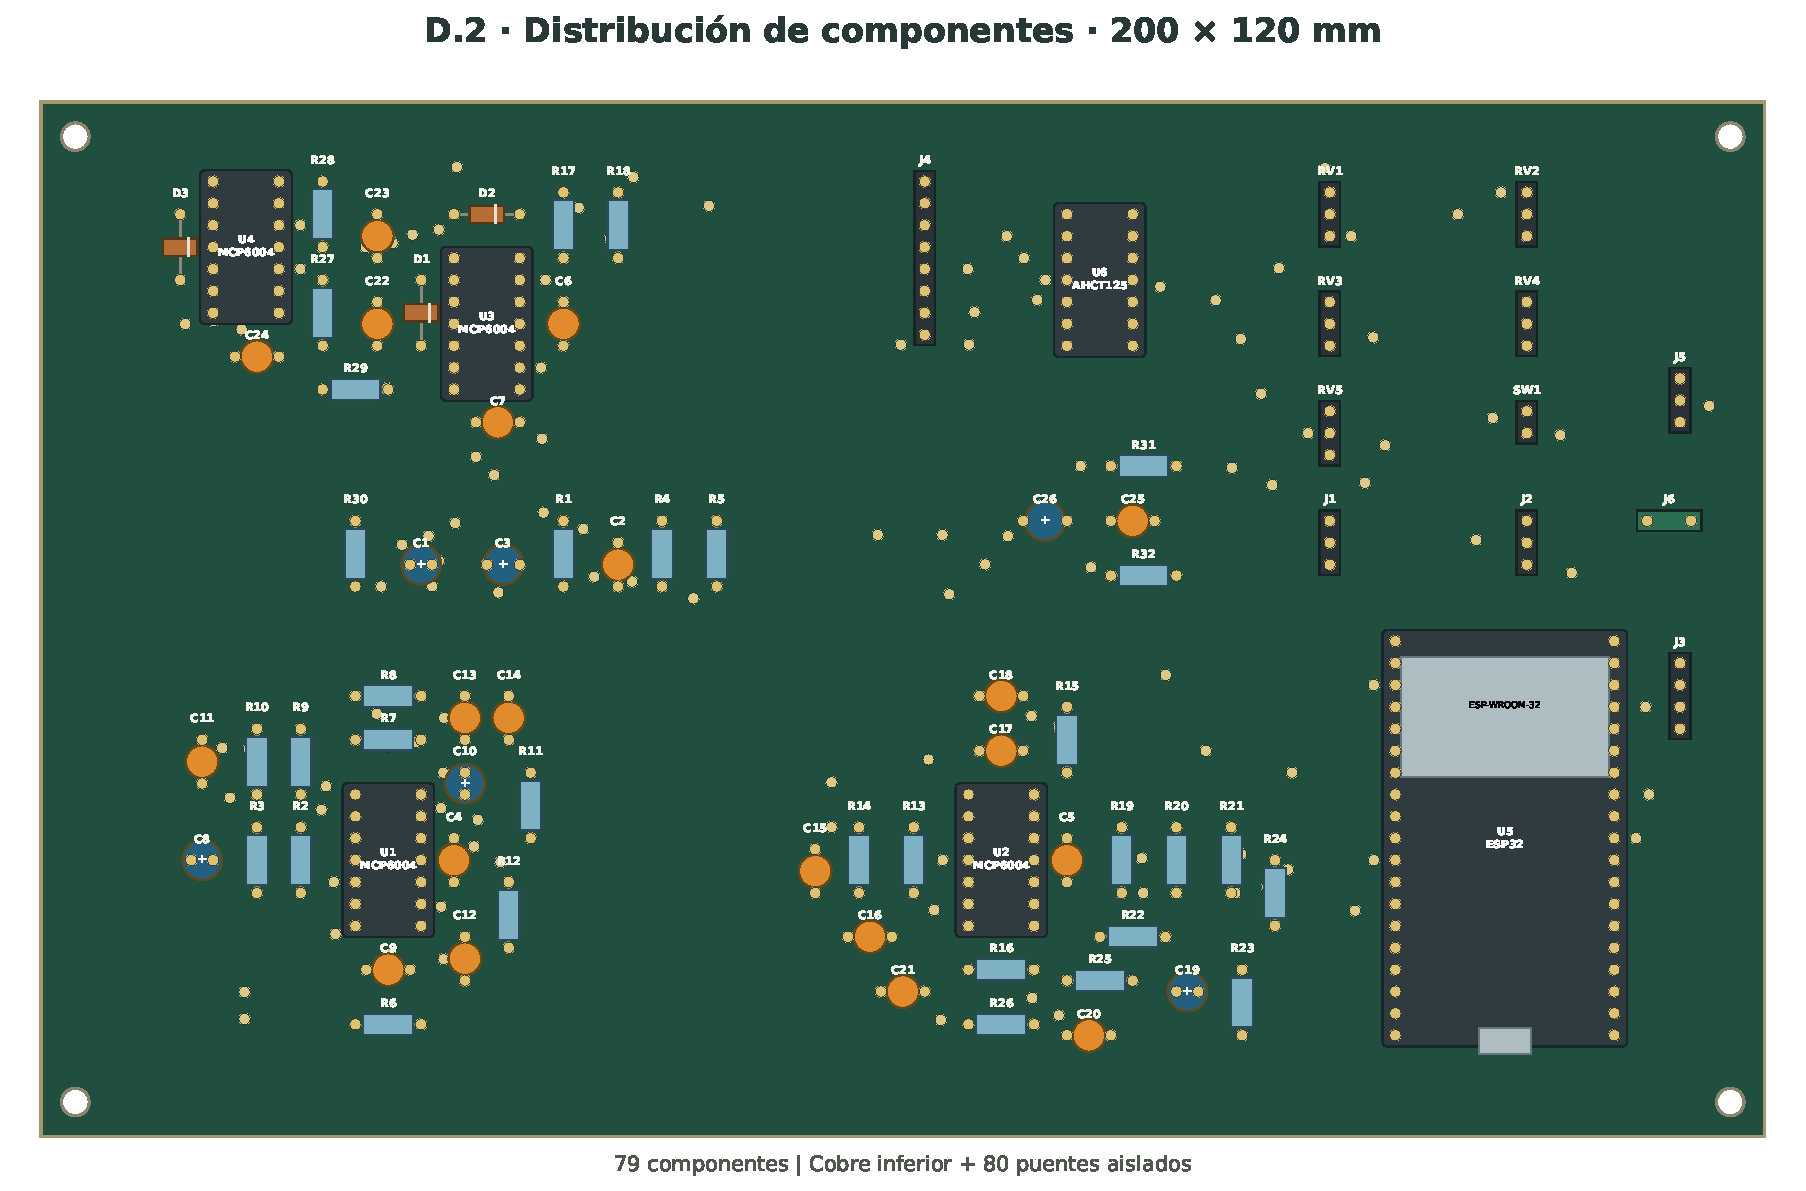
\includegraphics[width=\linewidth,height=5cm,keepaspectratio]{circuitos/pcb-capas.pdf}\end{column}\begin{column}{.27\textwidth}\small
200 × 120 mm\par 29 puentes arriba\par 51 cables por debajo\par\vspace{3mm}
J4: Waveshare.\par J5: tira LED.\par J6: fuente externa.\par Controles cableados al panel.\par\vspace{4mm}
\href{run:../../hardware/pcb-rev-D2.pdf}{\beamergotobutton{Abrir PCB PDF}}
\end{column}\end{columns}
\note{Solo B.Cu contiene pistas. Los cruces se resuelven con cables aislados soldados en sus puntos numerados. El archivo de fabricación contiene una sola capa de cobre.}
\end{frame}
\begin{frame}[t]{Distribución del panel y del gabinete}
\centering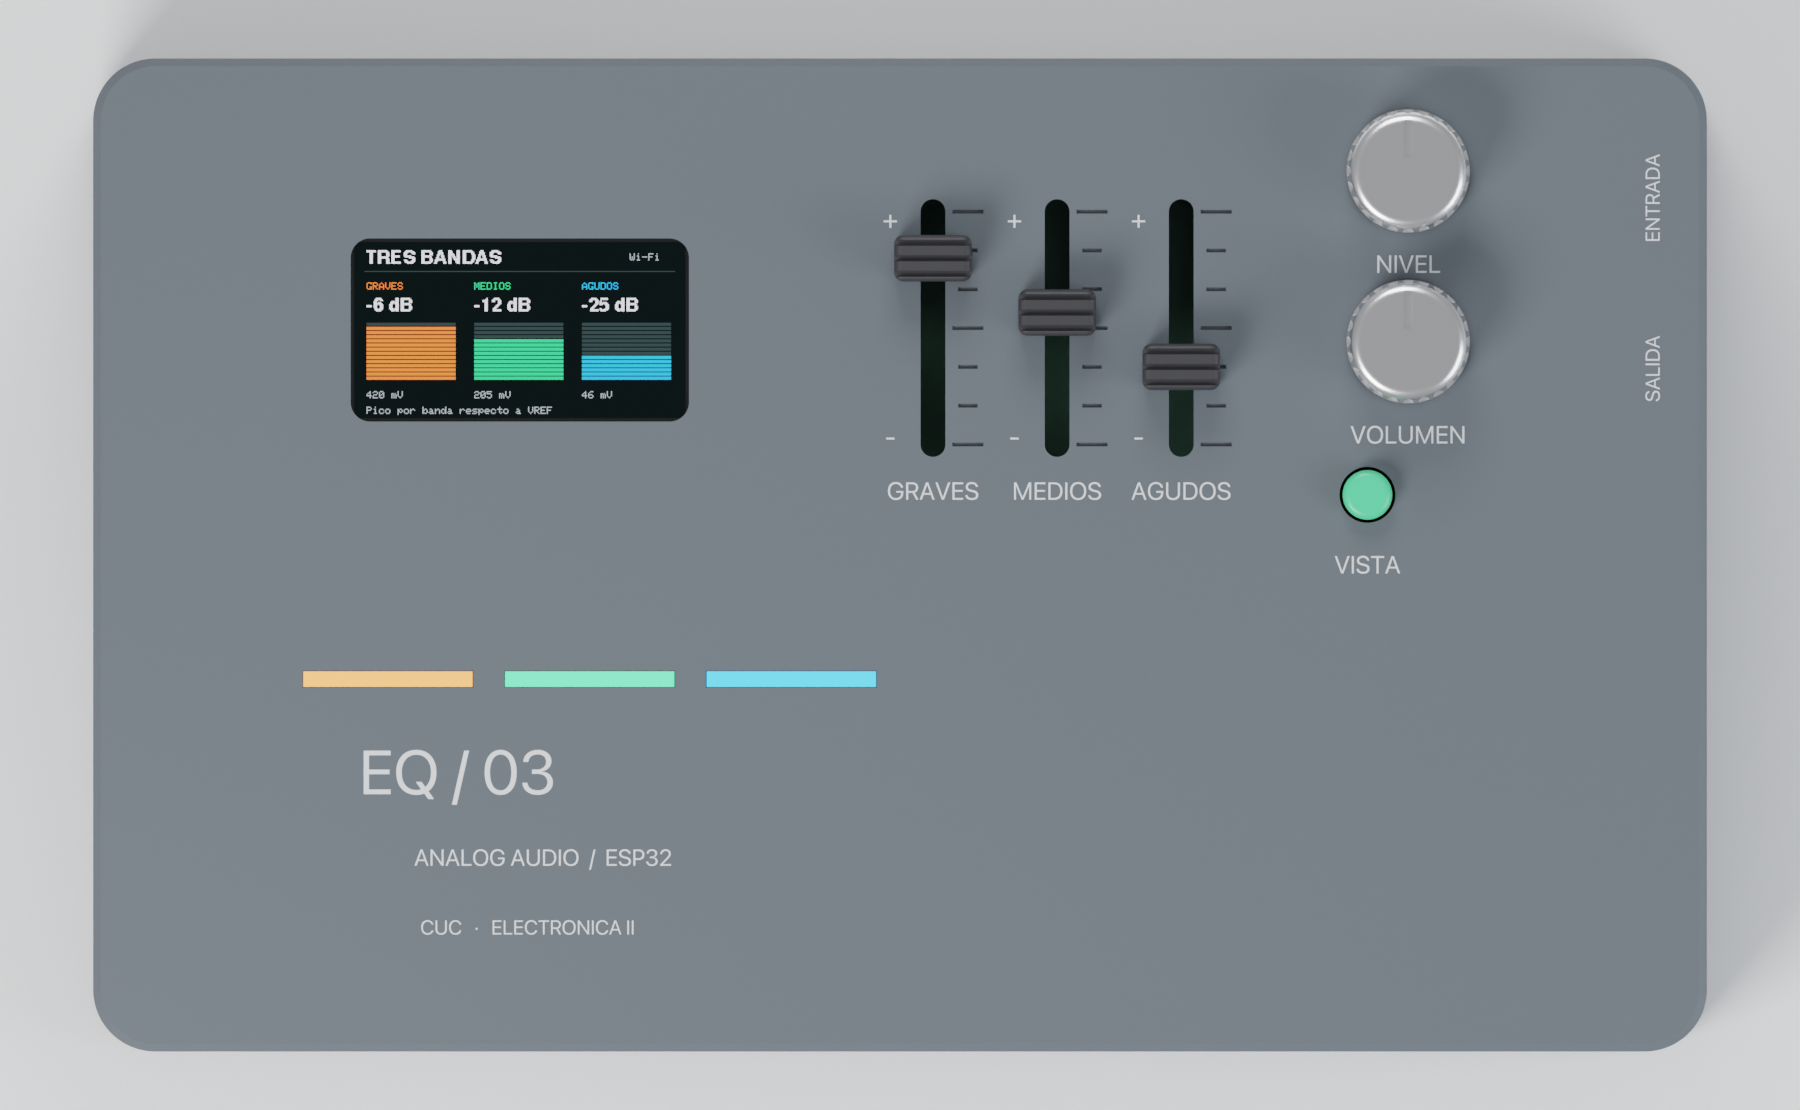
\includegraphics[width=\linewidth,height=4.9cm,keepaspectratio]{3d-gabinete-planta.png}\par\small 208 × 128 × 49,5 mm · acabado grafito · tapa magnética · canales LED.
\note{Los colores grises y las vistas abiertas y de planta siguen el criterio de los modelos de C2-ABPR. Las cotas del módulo real deben contrastarse antes de imprimir y montar.}
\end{frame}
\begin{frame}[t]{Tapa magnética, sin tornillos a la vista}
\begin{columns}[T]\begin{column}{.62\textwidth}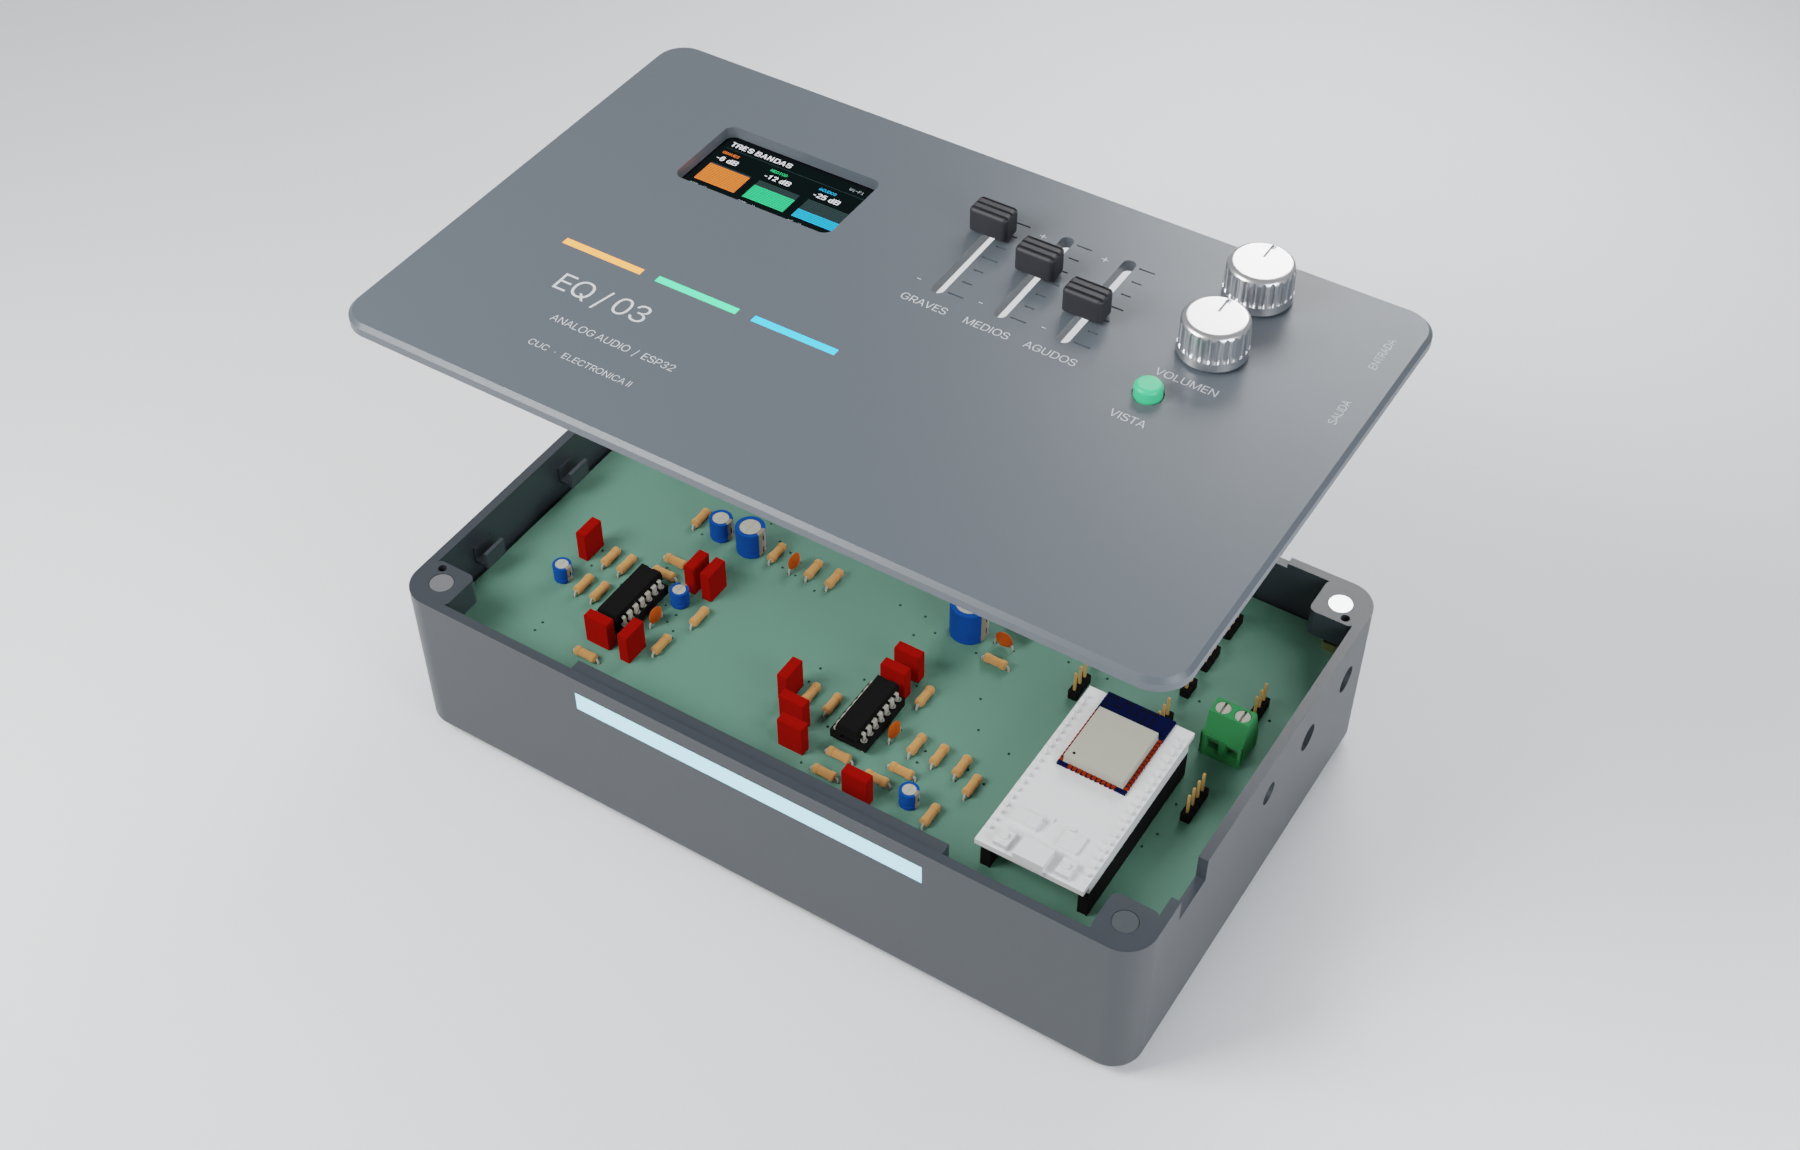
\includegraphics[width=\linewidth,height=5.2cm,keepaspectratio]{3d-gabinete-abierto.png}\end{column}\begin{column}{.34\textwidth}\small
Cuatro pares de imanes:\par \textbf{8 discos de Ø6 × 2 mm}.\par\vspace{3mm}
Alojamientos Ø6,3 × 2,2 mm.\par Techo de tapa: 0,8 mm.\par\vspace{3mm}
Dos guías de registro y un uñero posterior.\par\vspace{3mm}
La PCB conserva fijación mecánica independiente.
\end{column}\end{columns}
\note{Comprobar la polaridad de cada par antes de pegar. La holgura y el adhesivo se validan con una pieza de prueba. La fuerza de retención y el ajuste deben comprobarse con la tapa y el cable de pantalla instalados; no se han medido todavía.}
\end{frame}
\begin{frame}[t]{Ensayo de hoy: generador y osciloscopio}
\begin{columns}[T]\begin{column}{.46\textwidth}
\textbf{Entrada PRE}\par Senoidal de 200 mV pico a pico.\par Offset: 1,65 V.\par\vspace{3mm}
CH1: PRE. CH2: salida del filtro.\par Masas al GND del circuito.\par\vspace{3mm}
100 Hz: graves.\par 1 kHz: medios.\par 8 kHz: agudos.
\end{column}\begin{column}{.50\textwidth}
\textbf{Qué explicar}\par Comparar amplitud y fase.\par $|H|=V_{pp,out}/V_{pp,in}$.\par\vspace{3mm}
En Velxio: clic derecho sobre el cable y \textit{Add to scope}.\par\vspace{3mm}\small Los operacionales de esta prueba son ideales. El ensayo físico debe usar el MCP6004 y alimentación de 3,3 V.
\end{column}\end{columns}
\note{Cargar filtros-1000Hz.vlx. El generador inyecta directamente en PRE; esta prueba aísla los filtros. Añadir PRE y la salida al osciloscopio. En el banco, no conectar la pinza de masa a VREF. Cambiar a 100 Hz y a 8 kHz para comparar las bandas.}
\end{frame}
\begin{frame}[t]{Velxio: tres tonos, tres bandas}
\begin{columns}[T]\begin{column}{.34\textwidth}
\textbf{Ejecutado en el navegador}\par\vspace{3mm}
100 Hz: graves.\par1 kHz: medios.\par8 kHz: agudos.\par\vspace{4mm}
Tres archivos \texttt{.vlx}\par con el motor SPICE activo.\par\vspace{4mm}\small Modelo de operacional ideal. Prueba de selectividad; no del equipo completo.
\end{column}\begin{column}{.63\textwidth}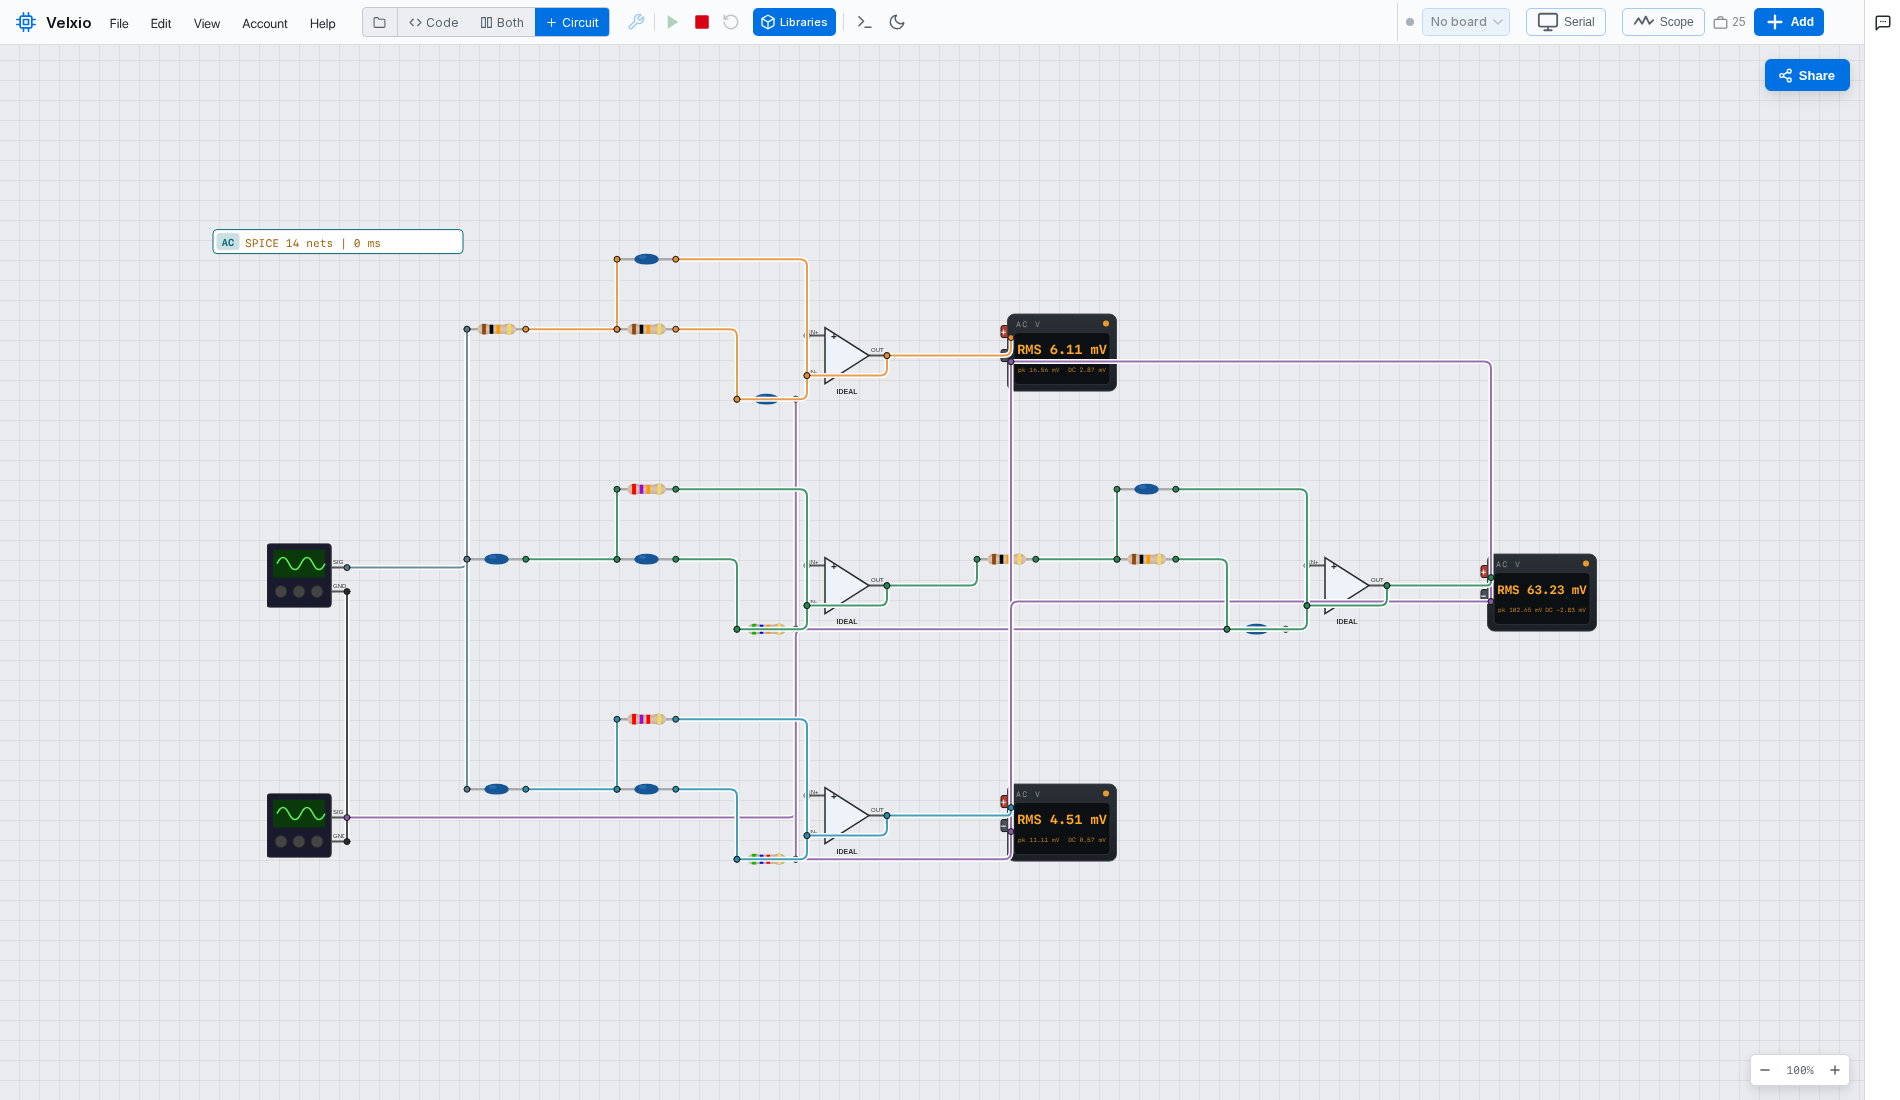
\includegraphics[width=\linewidth]{velxio-1000Hz.png}\end{column}\end{columns}
\note{Abrir File / Import project en Velxio y cargar uno de los tres archivos. Las lecturas RMS incluyen la ventana transitoria del simulador. En 1 kHz, medios registra 63,23 mV frente a 6,11 mV de graves y 4,51 mV de agudos. No atribuir al modelo ideal las limitaciones del MCP6004.}
\end{frame}
\begin{frame}[t]{Velxio: circuito, ESP32 y pantalla}
\begin{columns}[T]\begin{column}{.52\textwidth}
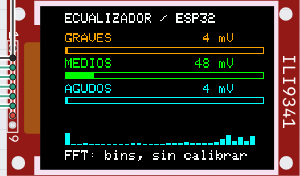
\includegraphics[width=\linewidth,height=3.7cm,keepaspectratio]{velxio-tft-1000Hz.png}\par\small Captura de la TFT con entrada de 1 kHz.
\end{column}\begin{column}{.44\textwidth}\small
Entrada $\rightarrow$ filtros $\rightarrow$ detectores $\rightarrow$ ADC $\rightarrow$ TFT.\par\vspace{3mm}
100 Hz: predominan graves.\par 1 kHz: predominan medios.\par 8 kHz: predominan agudos.\par\vspace{3mm}
\href{https://velxio.dev/editor?esp32sim=qemu}{\beamergotobutton{ABRIR VELXIO / QEMU}}\par\vspace{2mm}
Importar \texttt{integrado-1000Hz.vlx} y pulsar Run.
\end{column}\end{columns}\vspace{4mm}
\footnotesize TFT ILI9341 de sustitución; operacionales y diodos ideales. FFT sin calibración de frecuencia. El amplificador de potencia y los LED se ensayan aparte.
\note{Las barras proceden de analogRead ejecutado por el ESP32 emulado, no de una animación con amplitudes precargadas. Abrir el enlace con QEMU: el motor JavaScript aproxima las ondas del ADC a una constante. La TFT ILI9341 sustituye únicamente a la pantalla de esta simulación. No presentar la frecuencia calculada por la FFT como una medición válida; ese aspecto no quedó validado. Los proyectos y la guía INTEGRADO.md viajan en el paquete portátil y adjuntos al PDF.}
\end{frame}
\begin{frame}[t]{Ensayo animado de los 12 NeoPixel}
\begin{columns}[T]\begin{column}{.66\textwidth}
\only<1|handout:1>{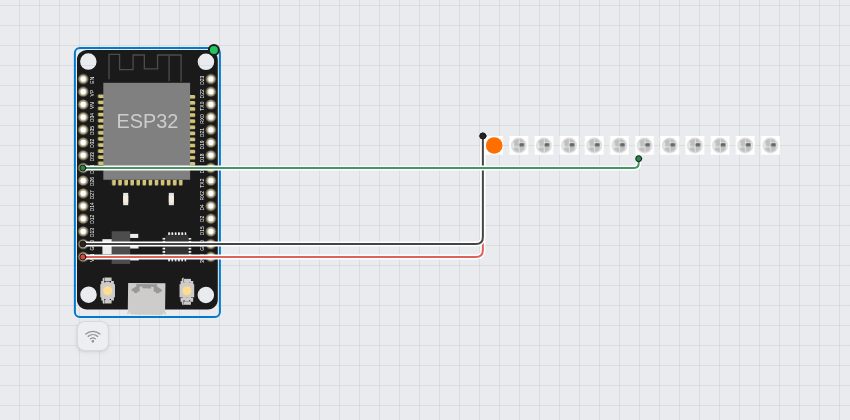
\includegraphics[width=\linewidth,height=4.7cm,keepaspectratio]{velxio-led-animado.png}}
\only<2|handout:0>{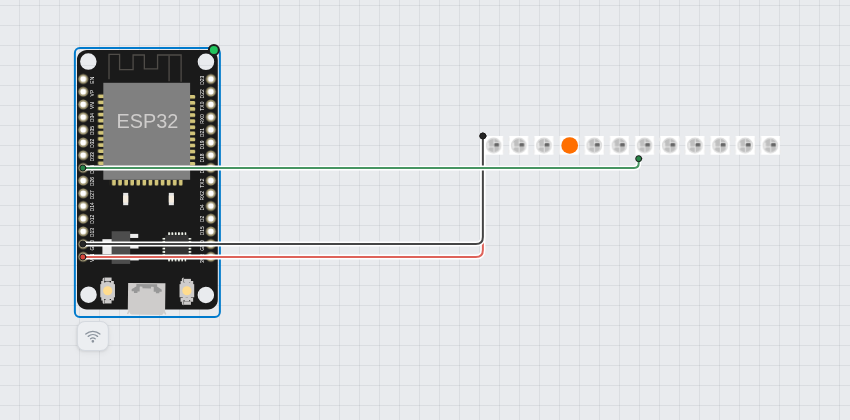
\includegraphics[width=\linewidth,height=4.7cm,keepaspectratio]{velxio-led-animado-2.png}}
\end{column}\begin{column}{.30\textwidth}\small
ESP32, GPIO25.\par Brillo 32/255.\par\vspace{3mm}
Cuatro LED naranjas, cuatro verdes y cuatro cian.\par\vspace{3mm}
La secuencia avanza cada 160 ms.\par\vspace{3mm}
\href{run:../../simulacion/velxio/index.html}{\beamergotobutton{Abrir ensayo LED}}\par\vspace{2mm}
Patrón programado sin entrada de audio.
\end{column}\end{columns}
\note{Importar led-animado.vlx y pulsar Run. Velxio compila el código del ESP32 y ejecuta la secuencia. Esta prueba comprueba el control y los colores; el adaptador AHCT, la corriente de la tira y el ruido sobre el audio se comprueban en el montaje físico.}
\end{frame}
\begin{frame}[t]{Abrir la simulación durante la exposición}
\begin{columns}[T]\begin{column}{.65\textwidth}
\href{https://velxio.dev/editor?esp32sim=qemu}{\beamergotobutton{ABRIR VELXIO}}
\par\vspace{5mm}\url{https://velxio.dev/editor?esp32sim=qemu}\par\vspace{5mm}
\small Descargar un caso y usar \textbf{File $\rightarrow$ Import project}.\par\vspace{3mm}
100 Hz $\rightarrow$ graves\par 1 kHz $\rightarrow$ medios\par 8 kHz $\rightarrow$ agudos\par Ensayo LED $\rightarrow$ pulsar Run\par\vspace{4mm}
\href{run:../../simulacion/velxio/index.html}{\beamergotobutton{Abrir carpeta de casos}}
\par\vspace{3mm}\footnotesize Los casos .vlx también van adjuntos al PDF.
\end{column}\begin{column}{.29\textwidth}
\includegraphics[width=\linewidth]{velxio-qr.png}\par\small QR: abre el editor.\par Importar después el caso.
\end{column}\end{columns}
\note{El enlace y el QR abren Velxio; no abren automáticamente un proyecto publicado. Los archivos están en simulacion/velxio y adjuntos al PDF. Tener el caso de 1 kHz descargado antes de la exposición. El visor PDF puede bloquear enlaces a archivos locales; en ese caso abrir index.html desde la carpeta del proyecto.}
\end{frame}
\begin{frame}[t]{Resultados de las comprobaciones}
\begin{tabularx}{\linewidth}{lX}\toprule
Comprobación & Resultado\\\midrule
Esquemático & ERC sin errores; 59 redes coinciden pin a pin.\\
PCB de una cara & Cobre inferior y 80 puentes; continuidad comprobada.\\
Filtros en Velxio & Graves a 100 Hz, medios a 1 kHz y agudos a 8 kHz.\\
Firmware & Compilación ESP32; pruebas DSP y dibujo por franjas.\\
Iluminación & Secuencia de 12 NeoPixel ejecutada por separado.\\\bottomrule
\end{tabularx}\vspace{5mm}\par Resultados obtenidos con herramientas de diseño y simulación.
\note{Mostrar cada registro junto a su herramienta. Los resultados analógicos, el ensayo LED y las pruebas del firmware tienen alcances distintos.}
\end{frame}
\begin{frame}[t]{Fuentes y archivos para la sustentación}
\small
\begin{itemize}
\item Texas Instruments: Sallen-Key, SLOA024B; 74AHCT125, SCLS264R.
\item Microchip: ficha técnica MCP6004.
\item Waveshare: ficha y esquema del módulo LCD de 1,9 pulgadas.
\item Analog Devices: ADAU1701. WLED: documentación Audio Reactive.
\item Adafruit: NeoPixel Überguide. Velxio: documentación del simulador.
\end{itemize}\vspace{5mm}
\normalsize\textbf{Repositorio}\par\url{https://github.com/davixcky/ecualizador-esp32}\vspace{4mm}\par Fuentes del informe y de esta presentación en \texttt{docs/latex/}.\par Resultados, esquemático, PCB y modelos 3D incluidos.
\note{Tener abiertos el informe de validación, el proyecto Velxio y el modelo 3D. Si preguntan por un valor, volver al cálculo y al nodo donde se verificó.}
\end{frame}
\begin{frame}[t]{Anexo: esquema completo para ampliar}
\hypertarget{esquemacompleto}{}
\centering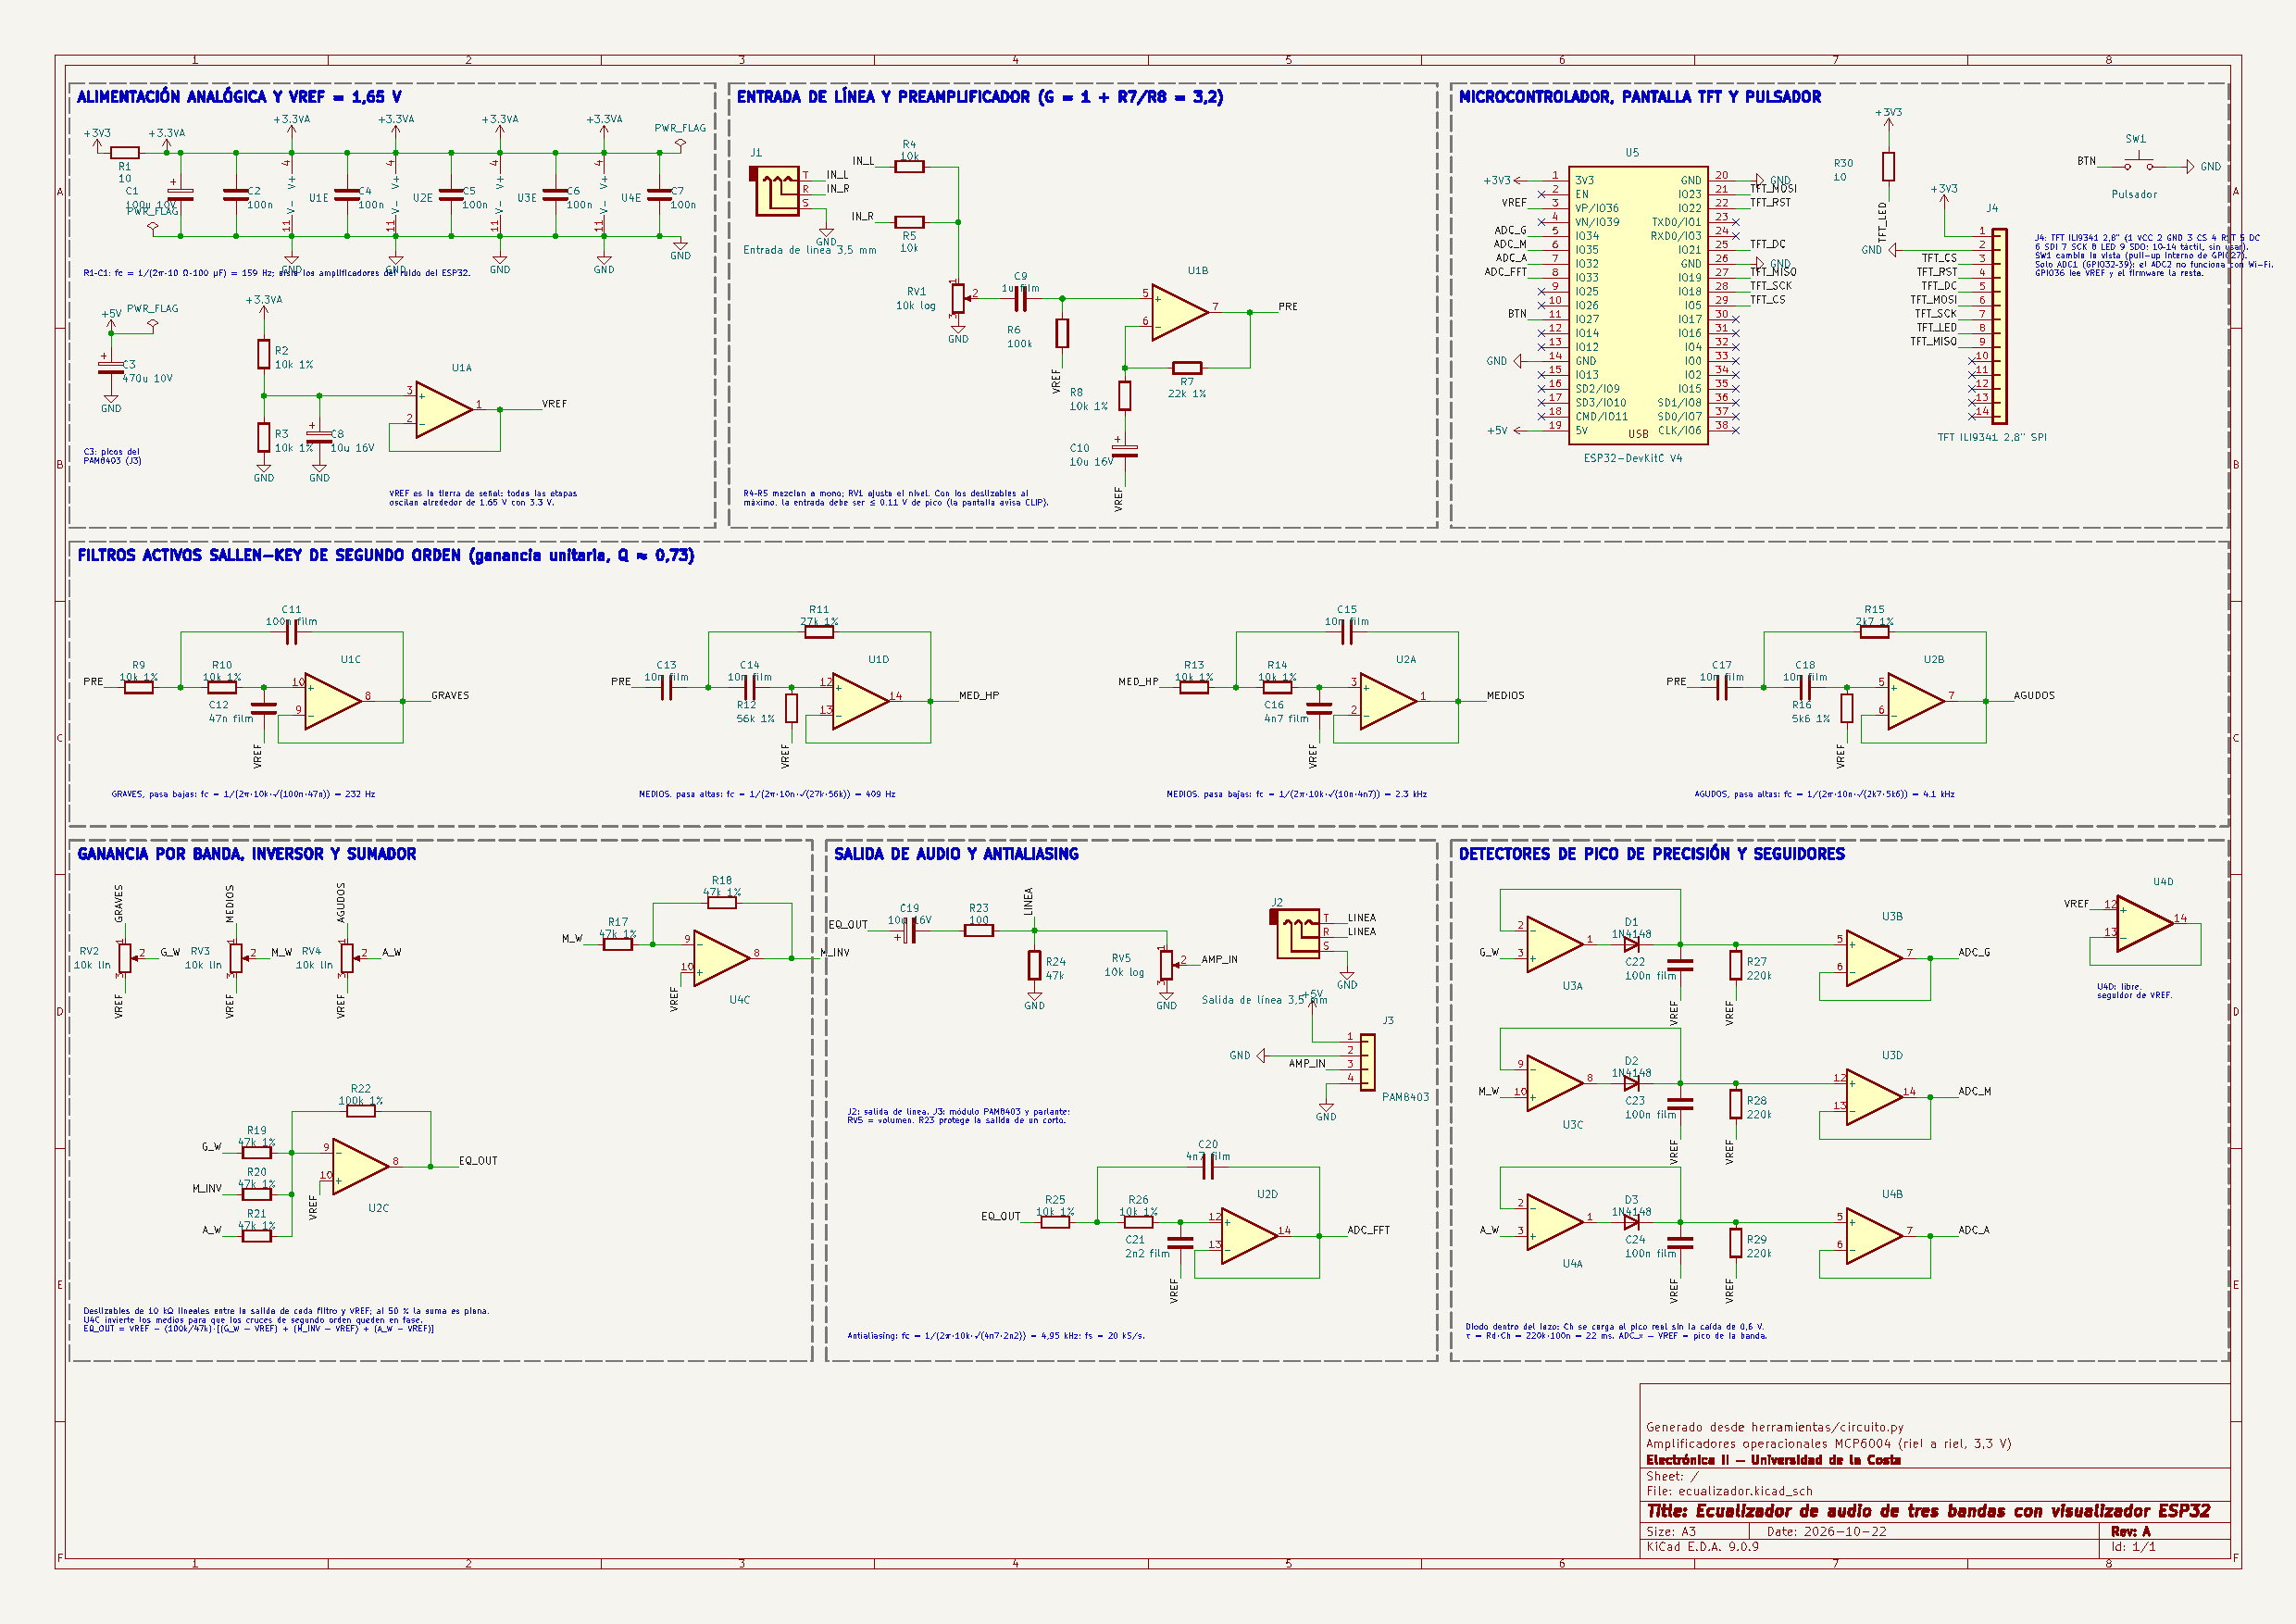
\includegraphics[width=\linewidth,height=5.2cm,keepaspectratio]{../../hardware/ecualizador.pdf}\par
\scriptsize El esquema está dentro de esta presentación. En PDF, ampliar con zoom; también se incluye como archivo independiente en el paquete para exposición.
\note{Esta página permite consultar el esquema sin depender de las carpetas del computador original. Para leer los valores pequeños, abrir el PDF de la presentación y ampliar esta página, o abrir esquema.pdf dentro del paquete de exposición.}
\end{frame}
\end{document}
